%%%%%%%%%%%%%%%%%%%%%%%%%%%%%%%%%%%%%%%%%
% Beamer Presentation
% LaTeX Template
% Version 1.0 (10/11/12)
%
% This template has been downloaded from:
% http://www.LaTeXTemplates.com
%
% License:
% CC BY-NC-SA 3.0 (http://creativecommons.org/licenses/by-nc-sa/3.0/)
%
%%%%%%%%%%%%%%%%%%%%%%%%%%%%%%%%%%%%%%%%%

%----------------------------------------------------------------------------------------
%	PACKAGES AND THEMES
%----------------------------------------------------------------------------------------

\documentclass{beamer}

\mode<presentation> {

% The Beamer class comes with a number of default slide themes
% which change the colors and layouts of slides. Below this is a list
% of all the themes, uncomment each in turn to see what they look like.

%\usetheme{default}
%\usetheme{AnnArbor}
%\usetheme{Antibes}
%\usetheme{Bergen}
%\usetheme{Berkeley}
%\usetheme{Berlin}
%\usetheme{Boadilla}
%\usetheme{CambridgeUS}
%\usetheme{Copenhagen}
%\usetheme{Darmstadt}
%\usetheme{Dresden}
%\usetheme{Frankfurt}
%\usetheme{Goettingen}
%\usetheme{Hannover}
%\usetheme{Ilmenau}
%\usetheme{JuanLesPins}
%\usetheme{Luebeck}
\usetheme{Madrid}
%\usetheme{Malmoe}
%\usetheme{Marburg}
%\usetheme{Montpellier}
%\usetheme{PaloAlto}
%\usetheme{Pittsburgh}
%\usetheme{Rochester}
%\usetheme{Singapore}
%\usetheme{Szeged}
%\usetheme{Warsaw}

% As well as themes, the Beamer class has a number of color themes
% for any slide theme. Uncomment each of these in turn to see how it
% changes the colors of your current slide theme.


\definecolor{BLACK}{rgb}{0, 0, 0} 
\definecolor{ERGgreen}{rgb}{0.45, 0.61, 0.00} 
\definecolor{ERGblue}{rgb}{0.04706, 0.13725, 0.26667}
\definecolor{ERGlightblue}{rgb}{0.0, 0.58, 0.71} 
\definecolor{ERGred}{rgb}{0.8, 0.00, 0.00} 
\definecolor{ERGyellow}{rgb}{0.9, 0.75, 0.0} 

\usecolortheme[named=ERGblue]{structure}
\newcommand{\quotes}[1]{``#1''}

%\usecolortheme{albatross}
%\usecolortheme{beaver}
%\usecolortheme{beetle}
%\usecolortheme{crane}
%\usecolortheme{dolphin}
%\usecolortheme{dove}
%\usecolortheme{fly}
%\usecolortheme{lily}
%\usecolortheme{orchid}
%\usecolortheme{rose}
%\usecolortheme{seagull}
%\usecolortheme{seahorse}
%\usecolortheme{whale}
%\usecolortheme{wolverine}

%\setbeamertemplate{footline} % To remove the footer line in all slides uncomment this line
%\setbeamertemplate{footline}[page number] % To replace the footer line in all slides with a simple slide count uncomment this line

%\setbeamertemplate{navigation symbols}{} % To remove the navigation symbols from the bottom of all slides uncomment this line
}

\usepackage{graphicx} % Allows including images
\usepackage{booktabs} % Allows the use of \toprule, \midrule and \bottomrule in tables
\usepackage{subfigure}
\usepackage[italian,english]{babel}
\usepackage[utf8]{inputenc}
\usepackage{amsmath}
\usepackage[colorinlistoftodos]{todonotes}
\usepackage{xcolor}
\usepackage{bbm}
\usepackage{skull}
\usepackage{bbm}
\usepackage{fourier}
\usepackage{cancel}
\usepackage{booktabs}
\usepackage{tabularx}
\usepackage{lipsum}
\usepackage{tcolorbox}
\usepackage{natbib}
\usepackage{marvosym}
\usepackage{mathtools}
\usepackage{lipsum} 
\usepackage{hyperref}
\usepackage{amssymb}
\usepackage{pifont}
\usepackage[font=tiny,labelfont=bf]{caption}

\newcommand{\mail}[1]{\href{mailto:#1}{\texttt{#1}}}
%\usepackage[framed,numbered,autolinebreaks,useliterate]{mcode}
\newcommand{\cmark}{\ding{51}}%
\newcommand{\xmark}{\ding{55}}%


\usefonttheme{serif} % here, there are other solutions

\newcommand{\norm}[1]{\left\lVert#1\right\rVert}

\theoremstyle{plain}
\newtheorem{thm}{Theorem}[section]
\newtheorem{lem}[thm]{Lemma}
\newtheorem{prop}[thm]{Proposition}
\newtheorem{rmk}[thm]{Remark}
\newtheorem*{cor}{Corollary}

\theoremstyle{definition}
\newtheorem{defn}{Definition}[section]
\newtheorem{conj}{Conjecture}[section]
\newtheorem{exmp}{Example}[section]
\newtheorem{algo}{Algorithm}[section]

%% Definizione di Nuovi comandi
\newcommand{\E}{\mathbb{E}}
\newcommand{\Pb}{\mathbb{P}}
\newcommand{\pdf}{\textit{pdf}}
\newcommand{\chf}{\textit{chf}}

\DeclareMathOperator*{\argmax}{arg\,max}
\DeclareMathOperator*{\argmin}{arg\,min}

\newcommand\blfootnote[1]{%
  \begingroup
  \renewcommand\thefootnote{}\footnote{#1}%
  \addtocounter{footnote}{-1}%
  \endgroup
}




%----------------------------------------------------------------------------------------
%	TITLE PAGE
%----------------------------------------------------------------------------------------

\setbeamertemplate{caption}[numbered]

\title[Financial Engineering]{Historical vs Market Calibration}  % The short title appears at the bottom of every slide, the full title is only on the title page

\author{Matteo Gardini} % Your name
\institute[UniGe] % Your institution as it will appear on the bottom of every slide, may be shorthand to save space
{
{\large Università degli Studi di Genova} \\ % Your institution for the title page
%\medskip
%\textit{mgardini@erg.eu, gardini@dima.unige.it} % Your email address
}
\date{Helsinki, 23 November 2022} % Date, can be changed to a custom date

\definecolor{darkgreen}{rgb}{0,0.5,0}
\definecolor{darkred}{rgb}{0.5,0,0}
\definecolor{darkblue}{rgb}{0,0,0.5}
\definecolor{gold}{rgb}{1,0.8431,0}

\newtcolorbox{mybox}[3][]
{
  colframe = #2!25,
  colback  = #2!10,
  coltitle = #2!20!black,  
  title    = {#3},
  #1,
}

\makeatletter
\newenvironment<>{proofs}[1][\proofname]
{%
	\par
	\def\insertproofname{#1\@addpunct{.}
}%
\usebeamertemplate{proof begin}#2}
{\usebeamertemplate{proof end}}
\makeatother

\begin{document}

\begin{frame}
\titlepage % Print the title page as the first slide
\begin{figure}

\includegraphics[width=0.20\textwidth]{UnigeLOGO}
\end{figure}
\end{frame}


%----------------------------------------------------------------------------------------
%	PRESENTATION SLIDES
%----------------------------------------------------------------------------------------

%----------------------
% SLIDE
%----------------------
\begin{frame}
	\frametitle{Who am I?}
	
	\begin{minipage}{0.5\textwidth}
		My name is Matteo, I work as Quantitative Analyst at Eni Plenitude, Italy. \\
		\vskip 1cm
		\mail{gardini@dima.unige.it}
	\end{minipage} \hfill
	\begin{minipage}{0.45\textwidth}
		% Show the image at item three and afterwards
		\begin{figure}
			% From https://i.imgur.com/AyzVOIO.jpg
			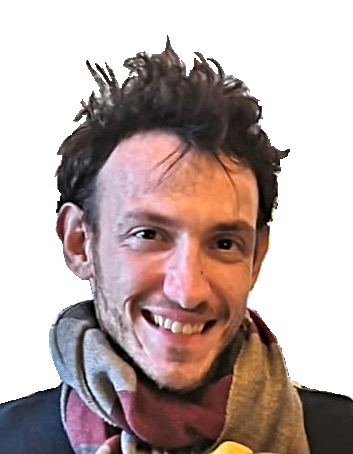
\includegraphics[height=0.9\textwidth]{ME.jpg}
			%\caption{Matteo Gardini}
		\end{figure}
	\end{minipage}
\end{frame}



%----------------------
% SLIDE
%----------------------
\begin{frame}
	\frametitle{Table of Contents}
	\tableofcontents
\end{frame}

\AtBeginSection[]
{
	\begin{frame}
		\frametitle{Table of Contents}
		\tableofcontents[currentsection]
	\end{frame}
}

%----------------------
% SLIDE
%----------------------
\begin{frame}
	\frametitle{Bibliography and references}
	Key concepts are contained in:
	\begin{itemize}
		\item \citet{Brigo2007}: gives a very useful overview of the topic and provides some \textit{ready to use} MATLAB code. It deals with \textbf{historical calibration} and \textbf{processes simulation}.
		\item \citet[Chapter 13]{CT2003}: it deals with \textbf{risk-neutral} calibration and provides a rich overview of Lévy processes applied to the mathematical finance.
	\end{itemize}
\end{frame}


%%%%%%%%%%%%%%%%%%%%%%%%%%%%%%%%%%%%%%%%%
\section{Calibration}
%%%%%%%%%%%%%%%%%%%%%%%%%%%%%%%%%%%%%%%%%

%----------------------
% SLIDE
%----------------------
\begin{frame}
\frametitle{Model Calibration}


\begin{mybox}{blue}{\textbf{Calibration}}
Once you defined a model for the market you have to \textbf{calibrate} it: this means you have to fit the parameters according to some real data.
\end{mybox}
\vspace{0.2cm}
This is a very important and delicate topic. Roughly speaking, calibrating a model leads to \textbf{solve a optimization problems}. Commonly used calibration techniques are:

\vspace{0.2cm}

\begin{itemize}
\item \textcolor{darkgreen}{Log-Likelihood estimation}.
\item \textcolor{darkgreen}{Least-Squares}.
\item Generalized Method of Moments.
\item Genetic Algorithms.
\item Kalman Filter.
\end{itemize}

\end{frame}

%----------------------
% SLIDE
%----------------------
\begin{frame}
	\frametitle{Model Calibration}
	
	
Why calibration is considered an hard-topic? Bacause:

\begin{itemize}
	\item Functional you have to minimize might be "highly non-linear" and might have several local minima: it is not guaranteed that a global minimum is reached.  
	\item Inverse problems are ill-posed: in particular the uniqueness of the solution is not guaranteed.
	\item Sophisticated optimization algorithms are required : most of them requires to compute the gradient of the objective function and this can be a really difficult task from a numerical point of view.
\end{itemize}
	
\end{frame}


%%%%%%%%%%%%%%%%%%%%%%%%%%%%%%%%%%%%%%%%%
\section{Historical Calibration - Maximum Likelihood Estimation}
%%%%%%%%%%%%%%%%%%%%%%%%%%%%%%%%%%%%%%%%%

%----------------------
% SLIDE
%----------------------
\begin{frame}
\frametitle{Historical Calibration - Maximum Likelihood Estimation}
The idea behind historical calibration is simple: \textit{given a set of observed data try to find a set of parameters that are \quotes{compatible} with the observed data in some sense}. Usually, a \textbf{Maximum Likelihood Estimation} (MLE) technique is used.
\vspace{0.2cm} 

\begin{defn}[Likelihood]
	Given a parameterized family of probability density functions  $f(x|\Theta)$ 
\begin{equation*}
	x \mapsto  f(x|\Theta)
\end{equation*}
where $\Theta$ is a parameter, the \textbf{likelihood function} is 
\begin{equation*}
	\Theta \mapsto  f(x|\Theta)
\end{equation*}
written $\mathcal{L}\left(\Theta\right) =   f(x|\Theta)$ where $x$ is the outcome of the experiment.
\end{defn}
Observe that the likelihood is not a probability density function.
\end{frame}



%----------------------
% SLIDE
%----------------------
\begin{frame}
	\frametitle{Historical Calibration - Maximum Likelihood Estimation}
	Consider the normal distribution and a given data-set $\boldsymbol{x}= \left(x_{1},\dots,x_{n}\right)$ of independent  realizations of an experiment. Then you have $\Theta= (\mu,\sigma)$ and the \emph{pdf} given by:
	\begin{equation*}
		f(x|\Theta) = \frac{1}{\sqrt{2 \pi \sigma^2}}e^{-\frac{(x-\mu)^{2}}{2\sigma}}
	\end{equation*}
we can say that the likelihood is $f(x|\Theta)$ regarded as a function of $\Theta$. If $\left\{x_{i}\right\}_{i\in \mathbb{N}}$ are i.i.d., then the likelihood of the random vector $\boldsymbol{x}$ is given by:

	\begin{equation*}
	\mathcal{L}\left(\Theta\right) \coloneqq f(\boldsymbol{x}|\Theta) = \prod_{i=1}^{n} \frac{1}{\sqrt{2 \pi \sigma^2}}e^{-\frac{(x_{i}-\mu)^{2}}{2\sigma}}.
\end{equation*}

\textbf{Exercize}: find the value of $\mu$ and $\sigma$ that maximize the likelihood $\mathcal{L}\left(\Theta\right)$.

\end{frame}


%----------------------
% SLIDE
%----------------------
\begin{frame}
	\frametitle{Historical Calibration - Maximum Likelihood Estimation}
	How to use this concept to calibrate a model? The idea is very simple:
	\vspace{0.5cm}
	\begin{mybox}{blue}{\textbf{Maximum Likelihood Estimation (intuitively)}}
	Find the set of parameter $\Theta$ such that, under the assumed statistical model, the observed data is most probable. The point in the parameter space that maximizes the likelihood function is called the \textit{maximum likelihood estimate}.
	In order to do so, maximize the likelihood $\mathcal{L}\left(\Theta\right)$ with respect to $\Theta$.
	\end{mybox}
\end{frame}

%----------------------
% SLIDE
%----------------------
\begin{frame}
\frametitle{Historical Calibration - Maximum Likelihood Estimation}
\begin{mybox}{darkgreen}{\textbf{Maximum Likelihood Estimation (formally)}}
Let $\mathcal{M}\left(\Theta\right)$ be a model and let $\Theta$ be its set of parameters. Let $\mathcal{L}\left(\Theta\right)$ be the likelihood of observing  a particular data sample. The $MLE$ estimate $\hat{\Theta}$ is such that:
\begin{equation*}
\hat{\Theta} = \argmax_{\Theta}\mathcal{L}\left(\Theta\right)
\end{equation*}
\end{mybox}

\begin{rmk}
	In order to apply this method, from a practical point of view, the likelihood function must be available is some \quotes{nice} form (as in the previous example). Under some model assumptions the likelihood assumes a simple form.
\end{rmk}
\end{frame}

%----------------------
% SLIDE
%----------------------
\begin{frame}
\frametitle{Historical Calibration - Maximum Likelihood for Lévy processes}
Now we show how to find the likelihood for Lévy processes ( see \citet{Brigo2007}).\\
\vspace{0.2cm}

Let $Y = \left\{Y(t);t\ge0\right\}$ be a Lévy process: we model the risky asset process $S = \left\{S(t);t\ge0\right\}$ as:
\begin{equation*}
	S(t) = S(0)e^{Y(t)}, \quad t \ge 0, \quad S(0) = S_{0}.
\end{equation*}
Assume to have a given data sample $x = \left(x_{1},x_{2},\dots,x_{n}\right)$\footnote{We state with $x_{i}$ the realization of the increment of the process $Y$ at time $t$, i.e. $x_{i} = X(t_{i}) \coloneqq Y(t_{i}) - Y(t_{i-1}) = \log S(t_{i}) - \log S(t_{i-1})$.}. In our example we suppose that the realization of the process $Y\left(t\right)$ are evenly spaces on a time grid $t_{0},t_{1},\dots,t_{n}$ where:
\begin{equation*}
	\Delta t = t_{i+1} - t_{i}.
\end{equation*}
\end{frame}


%----------------------
% SLIDE
%----------------------
\begin{frame}
	\frametitle{Historical Calibration - Maximum Likelihood for Lévy processes}
	Let be:
	\begin{equation*}
		X\left(t_{i}\right) \coloneqq \log S\left(t_{i}\right) - \log S\left(t_{i-1}\right).
	\end{equation*}
	By definition the likelihood function is:
	\begin{equation*}
		\mathcal{L}\left(\Theta\right) \coloneqq f_{X\left(t_{0}\right),\dots,X\left(t_{n}\right);\Theta}.
	\end{equation*}
	Since $X$ is a Markov process then:
	\begin{equation*}
		\begin{split}
			\mathcal{L}\left(\Theta\right) & = f_{X\left(t_{0}\right),\dots,X\left(t_{n}\right);\Theta}\\
			& = f_{X\left(t_{n}\right)|X\left(t_{n-1}\right);\Theta}\cdot f_{X\left(t_{n-1}\right)|X\left(t_{n-2}\right);\Theta} \cdot\; \dots \; \cdot  f_{X\left(t_{0}\right);\Theta}
		\end{split}
	\end{equation*}
	and, since the increments of $Y$ are i.i.d., it follows that 
	\begin{equation*}
		f_{X\left(t_{i}\right)|X\left(t_{i-1}\right);\Theta} = f_{X\left(t_{i}\right);\Theta},
	\end{equation*}
	and then:
	
	
\end{frame}



%----------------------
% SLIDE
%----------------------
\begin{frame}
	\frametitle{Historical Calibration - Maximum Likelihood for Lévy processes}
	\begin{equation*}
		\mathcal{L}\left(\Theta\right) = \prod_{i=1}^{n}f_{X\left(t_{i}\right);\Theta}.
	\end{equation*}
	
	Substituting the observed data set $x = \left(x_{1},\dots,x_{n}\right)$, we can write
	\begin{equation*}
		\mathcal{L}\left(\Theta\right) = \prod_{i=1}^{n}f_{\Theta}\left(x_{i}\right)
	\end{equation*}
	Since this product is very small numerical problems might arise when one tries to compute such a product. Then one usually maximize the following quantity: 
	\begin{equation*}
		\mathcal{L}^{*}\left(\Theta\right) = \log \mathcal{L}\left(\Theta\right) =  \sum_{i=1}^{n}\log f_{\Theta}\left(x_{i}\right)
	\end{equation*}
	
\end{frame}

%----------------------
% SLIDE
%----------------------
\begin{frame}
	\frametitle{Historical Calibration - Maximum Likelihood for Lévy processes}
	The set of parameters $\hat{\Theta}$ which maximizes the likelihood is obtained by solving:
	\begin{equation*}
	\hat{\Theta} = \max_{\Theta}\mathcal{L}^{*}\left(\Theta\right).
	\end{equation*}

\vspace{0.2cm}
Such a maximization can be done analytically only in some lucky situations (see for example the Black-Scholes model in \citet{Brigo2007}). Usually, some numerical techniques are used: \emph{MATLAB}, \emph{Python} and \emph{R} provide a lot of ready to use numerical algorithms.
\end{frame}


%----------------------
% SLIDE
%----------------------
\begin{frame}
\frametitle{Historical Calibration - Variance Gamma MLE}
How to apply MLE techniques to the Variance Gamma process? \\
\vspace{0.2cm}
Recall how the Variance Gamma process is defined. Assume that the log-prices of a given risky asset $S$ follow the dynamic:
\begin{equation*}
	d\log S(t) = \theta dg(t) + \sigma dW\left(g(t)\right), \quad S(0)=S_{0},\; t \ge 0.
\end{equation*}
where $\theta \in \mathbb{R}$, $\sigma \in \mathbb{R}^{+}$, $g=\left\{g(t); t\ge 0\right\}$ is a Gamma process  $g(t)\sim \Gamma(\frac{t}{\nu},\nu)$, $ \nu \in \mathbb{R}^{+}$ and $W$ is a standard Brownian motion independent of $g$. In this case the vector parameter we want to estimate is $\Theta= \left(\theta,\sigma,\nu\right)$.


\end{frame}



%----------------------
% SLIDE
%----------------------
\begin{frame}
\frametitle{Historical Calibration - Variance Gamma MLE}
Increments of Variance Gamma process are independent and, using the fact that conditioning with respect to $g(t)$ $d\log S(t)$ is Gaussian, it can be shown that:

\begin{equation}
	f_{\Theta}(x_{i}) = \frac{2e^{\frac{\theta x}{\sigma^{2}}}}{\sigma \sqrt{2\pi}\nu^{\Delta t/\nu}\Gamma(\frac{1}{\nu})} \left(\frac{|x|}{\sqrt{\frac{2\sigma^{2}}{\nu}+\theta^{2}}}\right)^{\frac{\Delta t}{\nu}-\frac{1}{2}}K_{\frac{\Delta t}{\nu}-\frac{1}{2}}\left(\frac{|s|\sqrt{\frac{2 \sigma^{2}}{\nu}+\theta^{2}}}{\sigma^{2}}\right)
	\label{eq:densityMLE}
\end{equation}
where $\Gamma(x)$ is the Gamma function and $K_{\eta}(\cdot)$ is the modified Bessel function of the Third kind.\\
\vspace{0.1cm}
\textcolor{darkgreen}{\textbf{Note}}: Gamma and Bessel functions can be computed numerically in a very efficient way.\\
\vspace{0.1cm}
\textcolor{darkgreen}{\textbf{Note}}: Equation \eqref{eq:densityMLE} seems to be an act of faith! See \citet{Brigo2007} for a brief explanation.\\
\vspace{0.1cm} 
\textbf{Exercise}: derive the expression in \eqref{eq:densityMLE}.

\end{frame}

%----------------------
% SLIDE
%----------------------
\begin{frame}
\frametitle{Historical Calibration - Variance Gamma MLE}
Now we can get the desired $\hat{\Theta}$ by numerically maximizing:
\begin{equation*}
	\mathcal{L}^{*}\left(\Theta\right) =  \sum_{i=1}^{n}\log f_{\Theta}\left(x_{i}\right)
\end{equation*}
Since  $\mathcal{L}^{*}\left(\Theta\right)$ is not linear local maxima can be present. 
Typically, most optimization algorithms need a starting point, say $\Theta_{0}$, to be run and the optimal value of $\mathcal{L}^{*}\left(\Theta\right)$  might depend on the chosen starting point. Is there a way to select a good starting point for the algorithm avoiding to pick it up randomly? \\


\vspace{0.2cm} 
\textbf{Exercise}: Take the code and try to change the starting point $\Theta_{0}$ of the minimization algorithm. What happens?

\end{frame}


%----------------------
% SLIDE
%----------------------
\begin{frame}
\frametitle{Historical Calibration - Variance Gamma MLE}
Remember that if $X$ is a Variance Gamma process with parameters $\theta,\sigma,\nu$ the Moment Generating Function $M_X(u), u \in \mathbb{R}$ is given by:
\begin{equation*}
	M_{X}(u) = \left(1 - \theta \nu u - \frac{1}{2}\nu \sigma^{2}u^{2}\right)^{-\frac{\Delta t}{\nu}}.
\end{equation*}
We can compute\footnote{$E[X^{n}] = M^{n}_{X}(0)$ where $M^{n}_{X}(0)$ is the $n$-th derivative of $M_X(u)$ computed at $0$.} the first four central moments:
\begin{align*}
& \mathbb{E}[X] = \theta \Delta t \\
& \mathbb{E}[(X - \mathbb{E}[X] )^{2}] = (\nu \theta^{2} + \sigma^{2})\Delta t \\
& \mathbb{E}[(X - \mathbb{E}[X] )^{3}]  = (2\theta^{3}\nu^{2} + 3 \sigma^{2}\nu \theta)\Delta t \\
& \mathbb{E}[(X - \mathbb{E}[X] )^{4}] = (3 \nu \sigma^2 + 12 \theta^2\sigma^2\nu^2 + 6 \theta^4 \nu^2)\Delta t + (3\sigma^{4} + 6 \theta^{2}\sigma^{2}\nu + 3 \theta^{4}\nu^{2})\Delta t^{2}.
\end{align*}


\end{frame}

%----------------------
% SLIDE
%----------------------
\begin{frame}
	\frametitle{Historical Calibration - Variance Gamma MLE}
We recall the definition of variance $V$, skewness $S$ and kurtosis $K$:
\begin{align*}
	 & M = \mathbb{E}[X]   & V  = \mathbb{E}[(X-\mathbb{E}[X] )^{2}] \\
	 & S  = \frac{\mathbb{E}[(X-\mathbb{E}[X] )^{3}]}{(\mathbb{E}[(X-\mathbb{E}[X] )^{2}])^{\frac{3}{2}}}
	&K  = \frac{\mathbb{E}[(X-\mathbb{E}[X] )^{4}]}{(\mathbb{E}[(X-\mathbb{E}[X] )^{2}])^{2}}
\end{align*}
All these quantity can be estimated from the data-set $x = (x_{i},\dots,x_{n})$\footnote{Recall that $x_{i} = \log S(t_{i}) - \log S(t_{i-1})$} and compared with the theoretical ones obtained from previous relations. If we assume that $\theta$ is \quotes{small} (as typically is in the applications) we get the following set for the starting point $\Theta_{0}$ of our optimization algorithm:
\begin{equation*}
	\sigma_{0} = \sqrt{\frac{V}{\Delta t}}, \quad \nu_{0} = \left(\frac{K}{3}-1\right)\Delta t, \quad \theta_{0}  = \frac{S\sigma \sqrt{\Delta t}}{3 \nu}. 
\end{equation*}
	
	
\end{frame}


%----------------------
% SLIDE
%----------------------
\begin{frame}
	\frametitle{Historical Calibration - Variance Gamma MLE}
	\begin{mybox}{blue}{\textbf{Maximum Likelihood Estimator}}
Now we can run the optimization algorithm and maximizing $\mathcal{L}(\Theta)$ with respect to $\Theta$ and obtaining the desired value $\hat{\Theta}$ which maximize the likelihood.
	\end{mybox}
\end{frame}

%----------------------
% SLIDE
%----------------------
\begin{frame}
	\frametitle{Historical Calibration - Variance Gamma MLE}
	\begin{mybox}{darkgreen}{\textbf{Generalized Method of Moments}}
	Roughly speaking, looking for the starting point $\Theta_{0}$ we have chosen parameters $\theta, \sigma$ and $\nu$ such that the moments are matched. Such a techniques is known as \textbf{Generalized Method of Moments} and it is a alternative way that can be adopted to calibrate our model.
	\end{mybox}
\end{frame}

%%----------------------
%% SLIDE
%%----------------------
%\begin{frame}
%	\frametitle{Historical Calibration - Variance Gamma MLE}
%	
%\end{frame}



\section{Risk Neutral Calibration}
%----------------------
% SLIDE
%----------------------
\begin{frame}
\frametitle{Risk Neutral Calibration - Introduction}

\begin{mybox}{blue}{\textbf{Risk-Neutral Calibration - Intuition}}
	Call option (and other derivatives contract in general) prices somehow reflect \quotes{the expectation of the behavior of the market of the future}. Historical quotations represent the past and, for this reason, \quotes{they do no give information about the future}.\\
	 If you want to price a derivative contract you must use the information about the future and, moreover, the price of the derivative you are valuing must be coherent with other quoted market products: in other words coherent means that \textbf{arbitrage opportunities must be avoided}.
\end{mybox}
\end{frame}

%----------------------
% SLIDE
%----------------------
\begin{frame}
	\frametitle{Risk Neutral Calibration - Introduction}
	In a Risk-neutral world the risky-asset is modeled as
	\begin{equation*}
		S(t) = S(0) e^{\omega t + rt + Y(t)}
	\end{equation*}
where $Y = \left\{Y(t);t\ge 0\right\}$ is a Lévy process, $r$ is the risk-free rate and $\omega$ is a parameter that must be chosen such that the discounted prices are martingales. Given the characteristic function of $Y$\footnote{$i = \sqrt{-1}$.}:

\begin{equation*}
\phi_{Y}(u) = \mathbb{E}[e^{iuY}] 
\end{equation*}
a simple way to get the martingale condition is to chose $\omega$ such that:
\begin{equation}
	\phi_{Y}(-i) = -\omega t.
	\label{eqn:riskneutrality}
\end{equation}
In the Variance Gamma condition \eqref{eqn:riskneutrality} leads to:
\begin{equation*}
	\omega= \frac{1}{\nu} \log\left(1 - \frac{\sigma^2 \nu}{2} - \theta \nu \right).
\end{equation*}

\end{frame}


\begin{frame}
	\frametitle{Risk Neutral Calibration - Idea}
Suppose we observe on the market $n$ European Call Options prices denoted with $C_{i}$ with $i=1,\dots,n$ having as underlying a given risky asset $S$. 
\vspace{0.1cm}
Denote with $\Theta$ the vector of unknown parameters and with  
$C_{i}^{\Theta}\left(K,T\right)$ the price in output from the chosen market model. The optimal $\hat{\Theta}$ can be found solving:

\begin{equation}
\hat{\Theta}  = \argmin_{\Theta} \sum_{i=1}^{n} \left(C_{i}^{\Theta}\left(K,T\right) - C_{i}\right)^{2},
\label{eqn:minimizationproblem}
\end{equation}
where: $C_{i}$ is the market price and $C_{i}^{\Theta}$ is the model price (which depends of course on $\Theta$).
\vspace{0,2cm}
\begin{mybox}{darkgreen}{\textbf{Intuitive explanation}}
This time we are looking for those set of parameters $\Theta$ such that the distance between model output prices $C_{i}^{\Theta}$  and market prices $C_{i}$ is minimum. 
\end{mybox}
\end{frame}

%----------------------
% SLIDE
%----------------------
\begin{frame}
	\frametitle{Risk Neutral Calibration - What do we need?}
We want to solve:
\begin{equation}
	\hat{\Theta} = \argmin_{\Theta} \sum_{i=1}^{n} \left(C_{i}^{\Theta}\left(K,T\right) - C_{i}\right)^{2}.
	\label{eqn:minimizationRN}
\end{equation}
Therefore we need, for the considered model $\mathcal{M}\left(\Theta\right)$, a way to compute $C_{i}^{\Theta}\left(K,T\right)$. Typically, fast methods to compute vanilla option prices (such as Call options) are available for many models. \\
\vspace{0.1cm} 
\par Since we have to use a minimization algorithm to solve the problem above and since optimization algorithms are generally iterative, the method we need to compute $C_{i}^{\Theta}\left(K,T\right)$ must be as fast as possible.


\end{frame}


%----------------------
% SLIDE
%----------------------
\begin{frame}
\frametitle{Risk Neutral Calibration - How to compute $C_{i}^{\Theta}\left(K,T\right)$?}
As stated above we need a numerically fast method to compute $C_{i}^{\Theta}\left(K,T\right)$.

\begin{itemize}
	\item Analytical formula \textcolor{darkgreen}{\cmark}.
	\item Monte Carlo Methods \textcolor{darkred}{\xmark}.
	\item Partial Differential Equation methods \textcolor{darkred}{\xmark}.
	\item Fourier Methods: FFT, Lewis, Convolution, COS and so on \textcolor{darkgreen}{\cmark}.
\end{itemize}

Analytical or semi-analytical formulas are not always available, but Fourier Methods can be used for almost all Lévy models.
\vspace{0.3cm}
\begin{mybox}{darkgreen}{\textbf{Conclusion}}
	At the end of procedure we have the parameter $\hat{\Theta}$ that minimize \eqref{eqn:minimizationRN} and hence the model $\mathcal{M}\left(\Theta\right)$ is calibrated. 
\end{mybox}

\end{frame}


%----------------------
% SLIDE
%----------------------
\begin{frame}
	\frametitle{Risk Neutral Calibration - Variance Gamma}
For the variance Gamma model a semi-analytic closed formula for Call options is available and it is given by:
\begin{equation}
	C^{\Theta}\left(K,T\right) = \int_{0}^{\infty}C(g)\frac{\frac{1}{\nu}^{\frac{t}{\nu}}}{\Gamma\left(\frac{t}{\nu}\right)}g^{\frac{t}{\nu}-1}e^{\frac{-g}{\nu}}
	\label{eqn:VGclosedformula}
\end{equation}
where $C\left(g\right)$ is the price of a Call within the Black-Scholes model. Integral in Equation \eqref{eqn:VGclosedformula} seems to be scaring but, actually, can be computed in a very efficient way using Bessel functions and Hypergeometric degenerated function as was shown by \citet{MadanSeneta90}. \\
\vspace{0.2cm}
\textcolor{darkred}{\textbf{Obs:}} In the following numerical experiment we do not use the explicit formula but the FFT method to compute the call option price $C^{\Theta}\left(K,T\right)$. This because FFT method can be applied to other Lévy models and hence it is a widely used method!

\end{frame}



\section{Numerical Application - Variance Gamma}
%----------------------
% SLIDE
%----------------------
\begin{frame}
	\frametitle{Numerical Application - Variance Gamma}	
Now we apply all methods analyzed before to a real case. We focus on Power Germany Future price. The outline is the following:
\begin{enumerate}
	\item We check that Lévy modeling is suitable.
	\item We Calibrate the Variance Gamma model on historical future prices.
	\item We Calibrate the Variance Gamma model on quoted Call options written on power Germany future prices.
	\item We compare the obtained results.
\end{enumerate}

\vspace{0.2cm}
We assume a risk-free rate of $r=0.01$. 

\end{frame}


%----------------------
% SLIDE
%----------------------
\begin{frame}
	\frametitle{Numerical Application - German Power future historical quotations}	
	\begin{figure}
		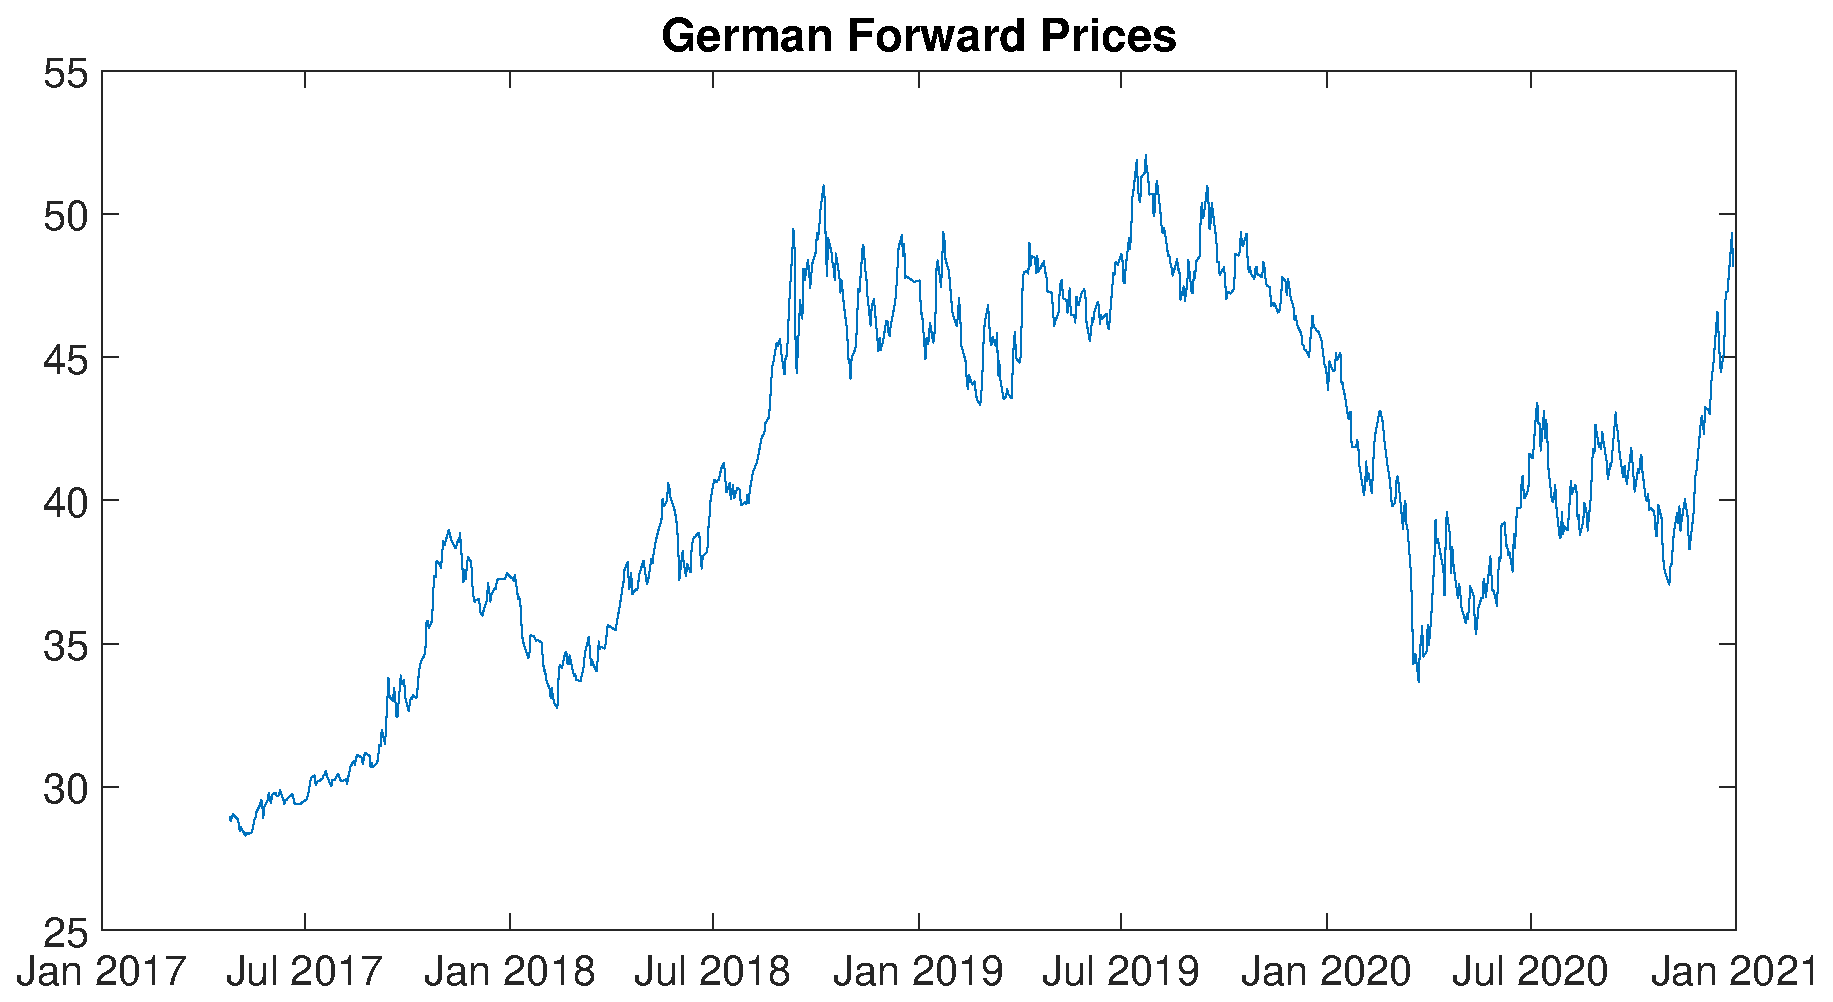
\includegraphics[scale=0.35]{images/HistoricalSeries.eps}
		\caption{Historical German Power Future quotations.}
	\end{figure}
\end{frame}

%----------------------
% SLIDE
%----------------------
\begin{frame}
	\frametitle{Numerical Application - Independence of increments}	
	First of all we have to check that increments (i.e. log-returns) of $n$ log-price process realizations are independent. There are several way to do so. One possible way is to plot the so called \textit{Autocorrelation function} of lag $k$ defined as:
	\begin{equation*}
		ACF(k) = \frac{1}{(n-k)\hat{v}} \sum_{i=1}^{n-k}(x_{i}-\hat{m})(x_{i}+k-\hat{m}),\quad k=1,2,\dots
	\end{equation*}
where $\hat{m}$ and $\hat{v}$ are the sample mean and variance of the series, respectively. $ACF(k)$ gives an estimate of the correlation between $X(t_{i})$ and $X(t_{i+k})$. If we want to use Lévy modeling framework we must observe a low level of increments correlation\footnote{Use the function \textit{autocorr} in \textit{MATLAB}.}.
\end{frame}

%----------------------
% SLIDE
%----------------------
\begin{frame}
	\frametitle{Numerical Application - Independence of increments}	
	\begin{figure}
	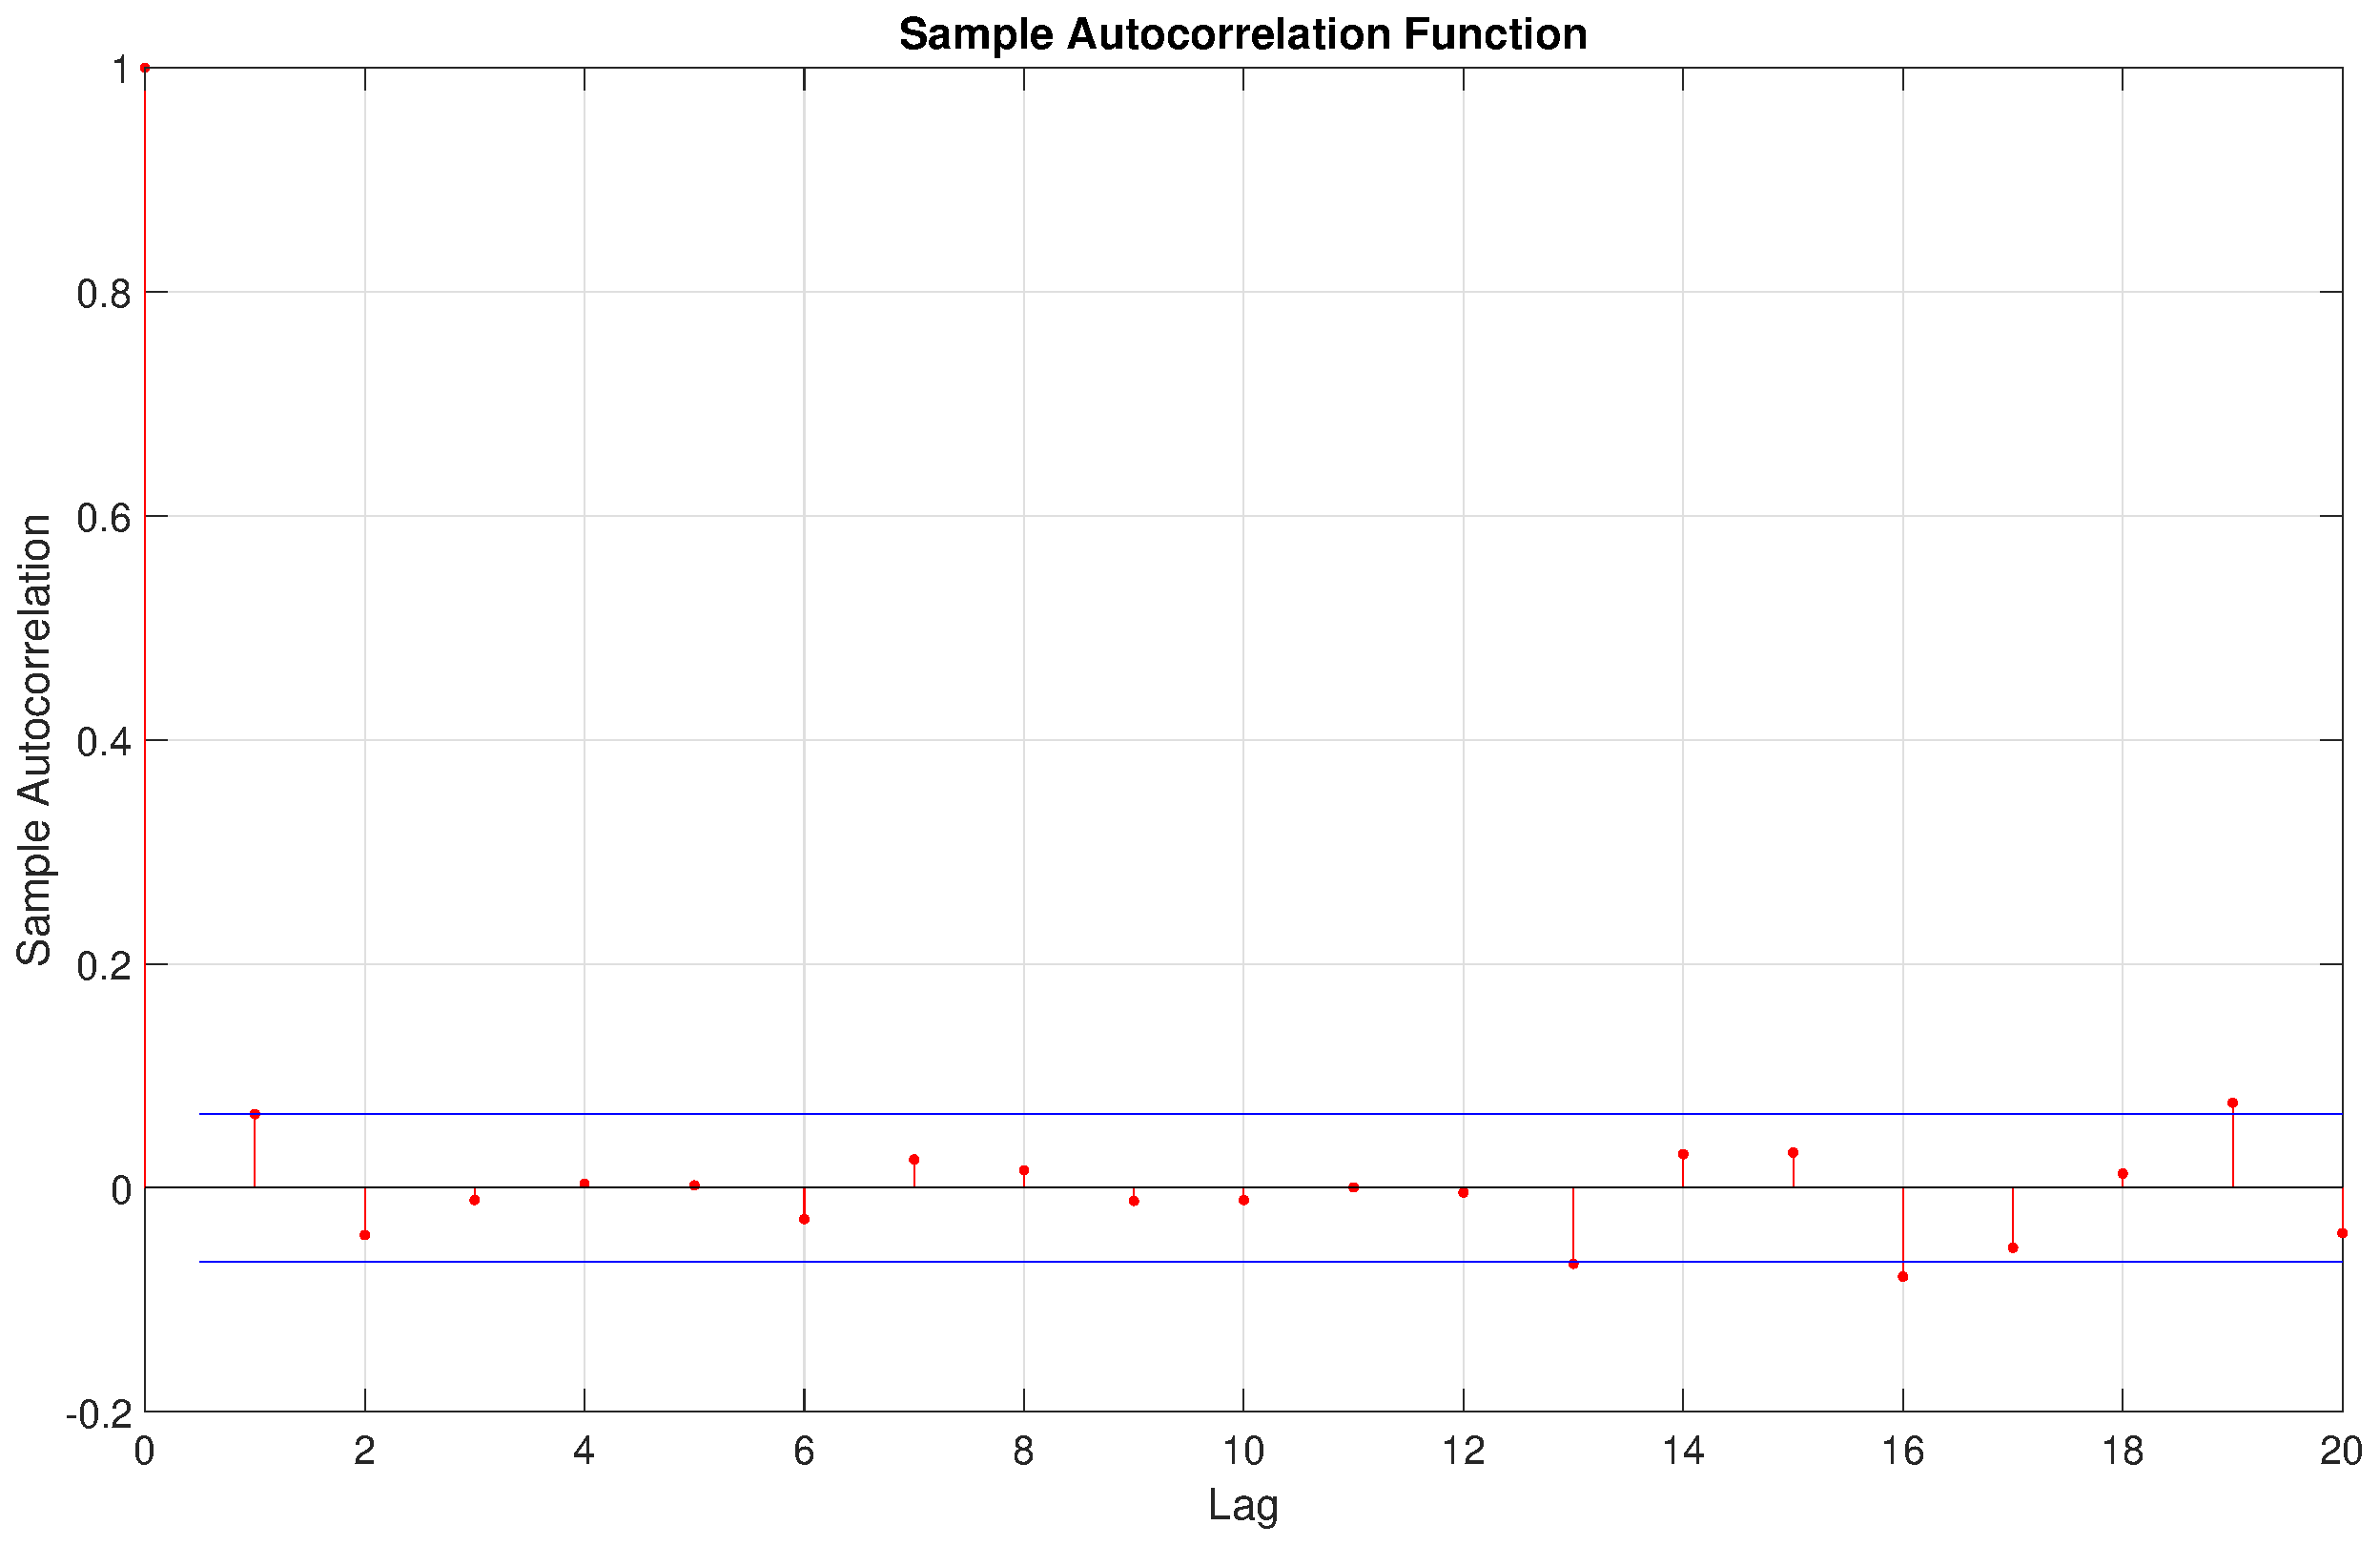
\includegraphics[scale=0.2]{images/Autocorrelation.eps}
	\caption{We see that no auto-regressive component in log-returns seems to be present. A Lévy process should be okay for modeling purposes.}
	\end{figure}
\end{frame}

%----------------------
% SLIDE
%----------------------
\begin{frame}
	\frametitle{Numerical Application - Which Lévy process?}
	Now we have to choose the \quotes{right} Lévy process to model the log-return process. 	To check the normality of log-returns we can use the QQ-plot (use \textit{qqplot} function in \textit{MATLAB}.)
	
		\begin{figure}
		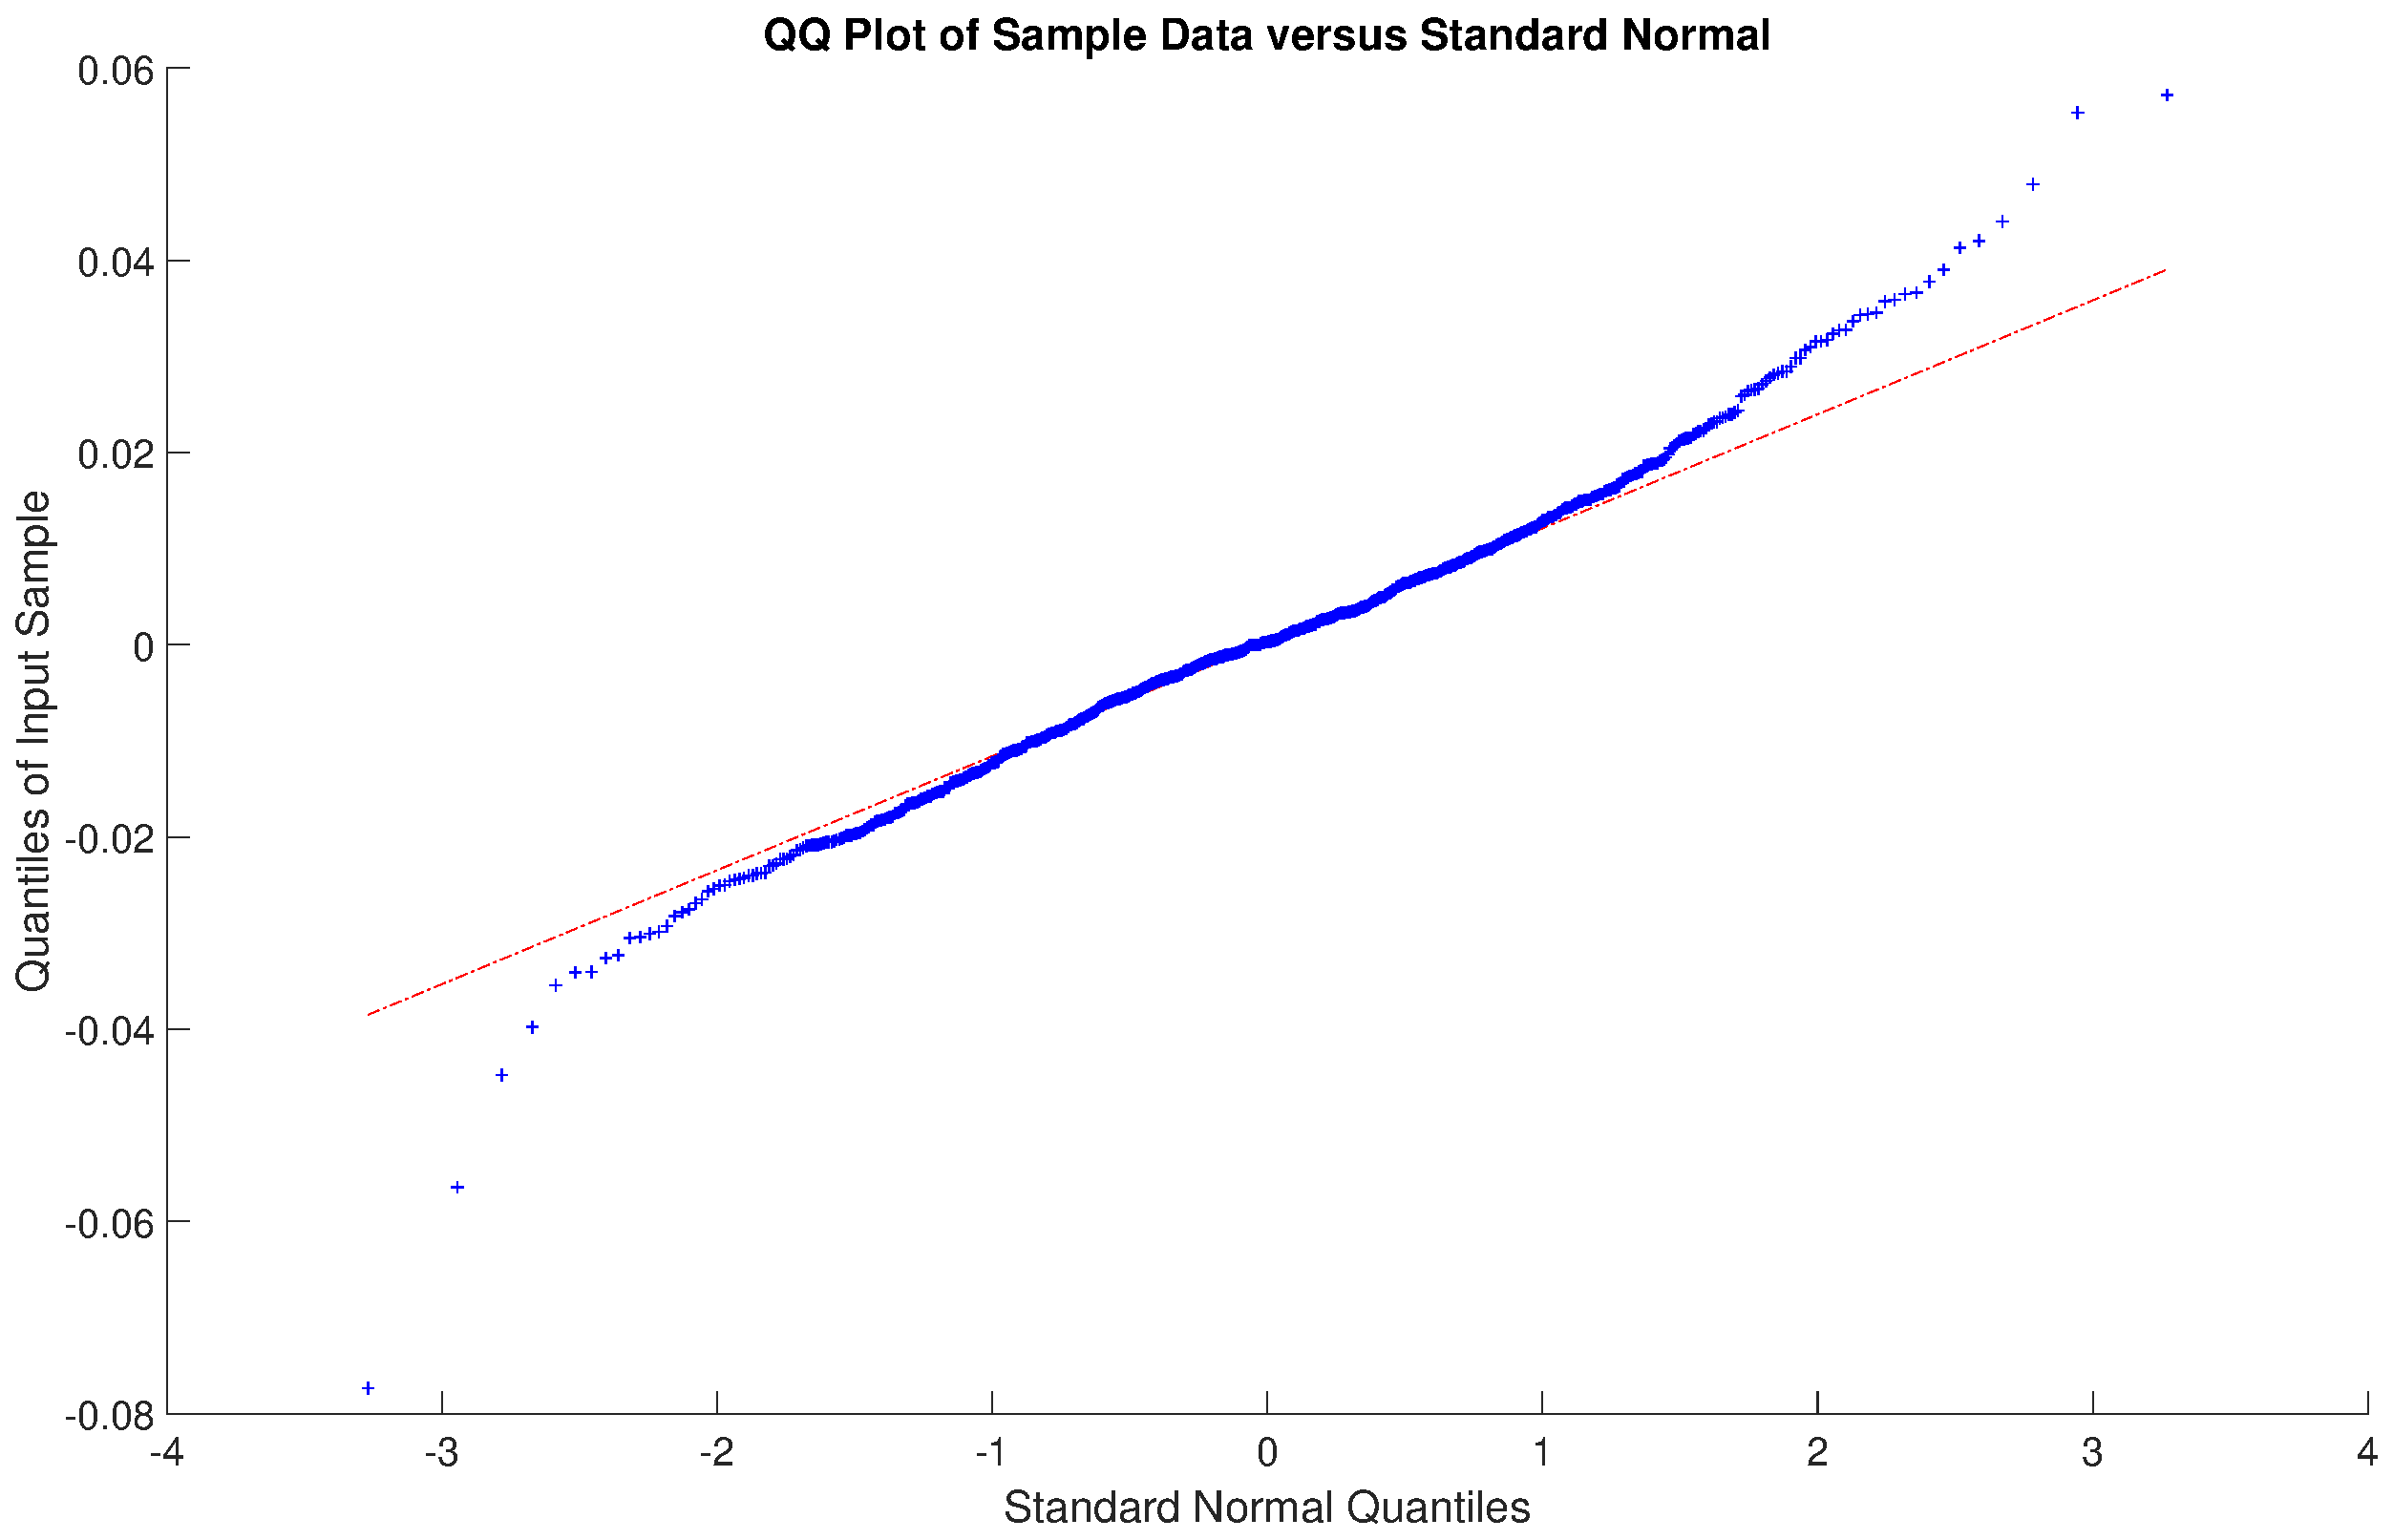
\includegraphics[scale=0.15]{images/QQplot.eps}
		\caption{The QQ-plot shows that the historical quantiles in the tail of the distribution are significantly larger compared to the normal distribution.}
	\end{figure}

Using the Black-Scholes model might be to narrow: hence we use the Variance-Gamma process.
	
\end{frame}

%----------------------
% SLIDE
%----------------------
\begin{frame}
	\frametitle{Numerical Application - Historical Calibration}	

\begin{table}[ht]
	\centering
	\begin{tabular}{c c c}
		\hline\hline
		$\theta$ & $\sigma$ & $\nu$ \\ [0.5ex] % inserts table %heading
		\hline
		0.1873 & 0.1917 & 0.002 \\ [1ex]
		\hline
	\end{tabular}
	\caption{Historical calibration of the Variance Gamma model using the MLE estimator.}
\end{table}

\begin{figure}
	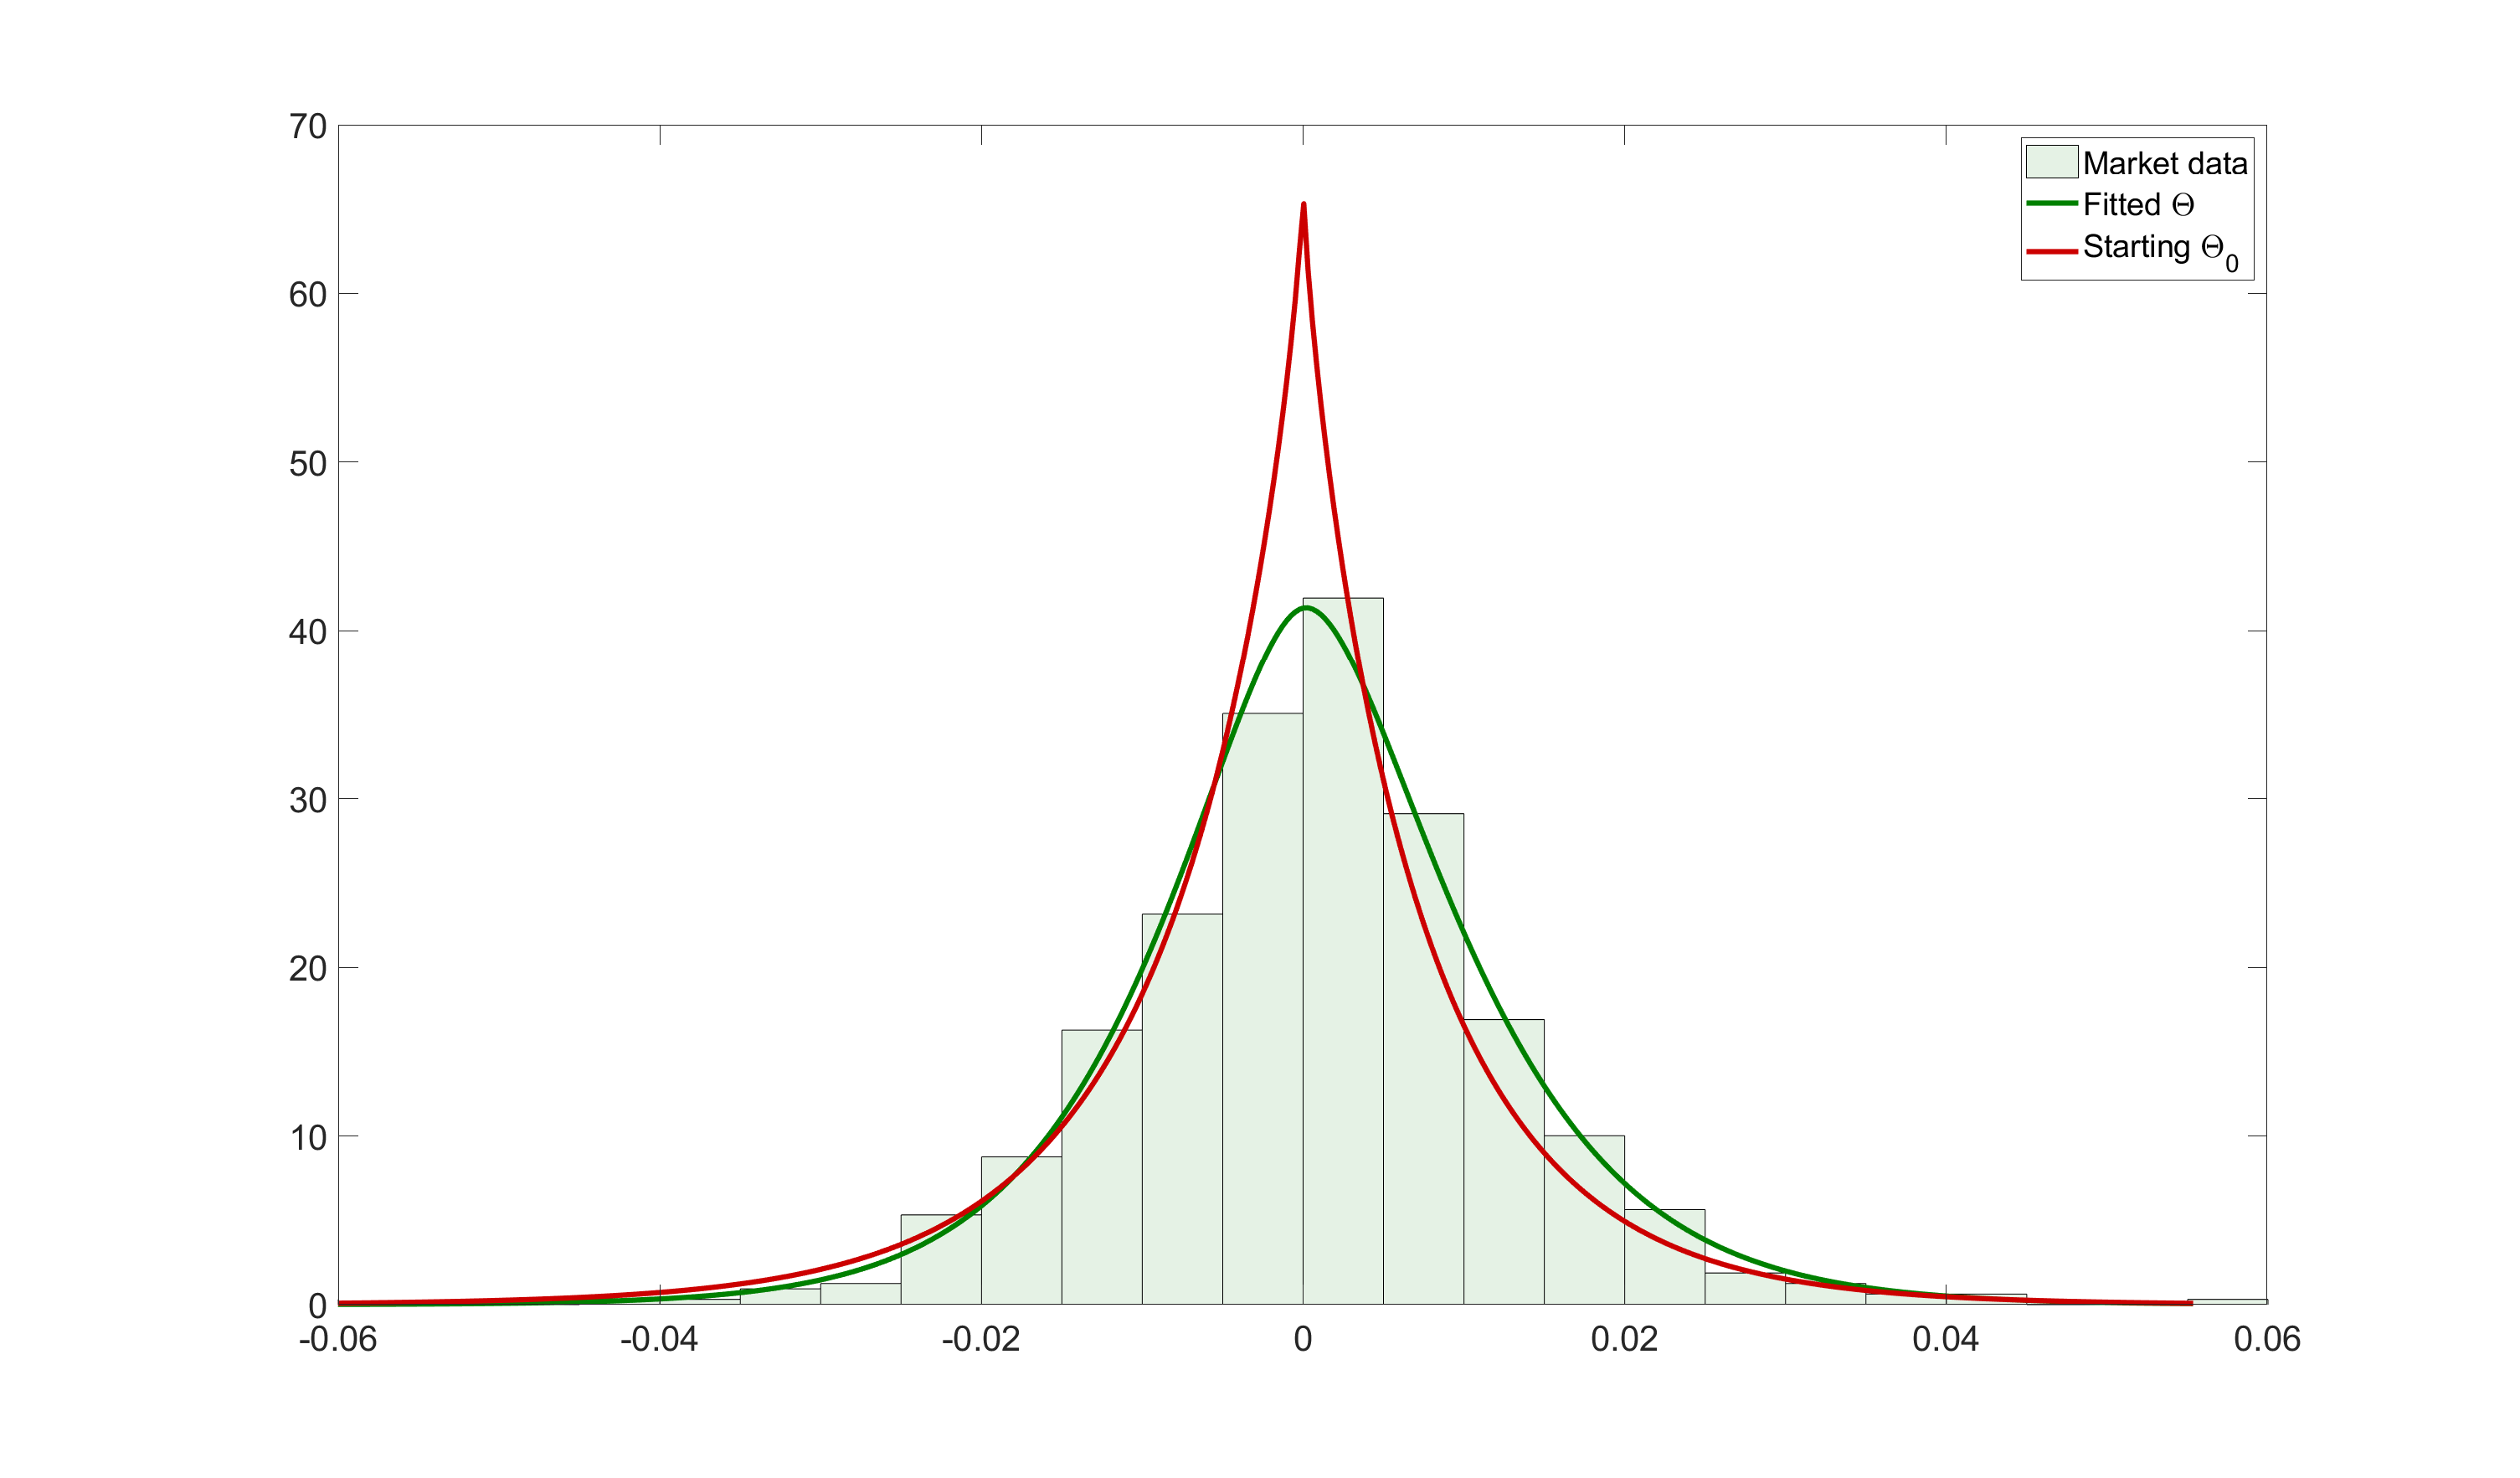
\includegraphics[scale=0.15]{images/FittingHistorical.eps}
	\caption{Fitted distribution compared to the historical one.}
\end{figure}


\end{frame}

%----------------------
% SLIDE
%----------------------
\begin{frame}
	\frametitle{Numerical Application - Risk-Neutral Calibration}	
	
	\begin{table}[ht]
		\centering
		\begin{tabular}{c c c}
			\hline\hline
			$\theta$ & $\sigma$ & $\nu$ \\ [0.5ex] % inserts table %heading
			\hline
			0.0900 & 0.2220 & 0.2231 \\ [1ex]
			\hline
		\end{tabular}
		\caption{Risk-Neutral calibration of the Variance Gamma model.}
	\end{table}
	
	\begin{figure}
		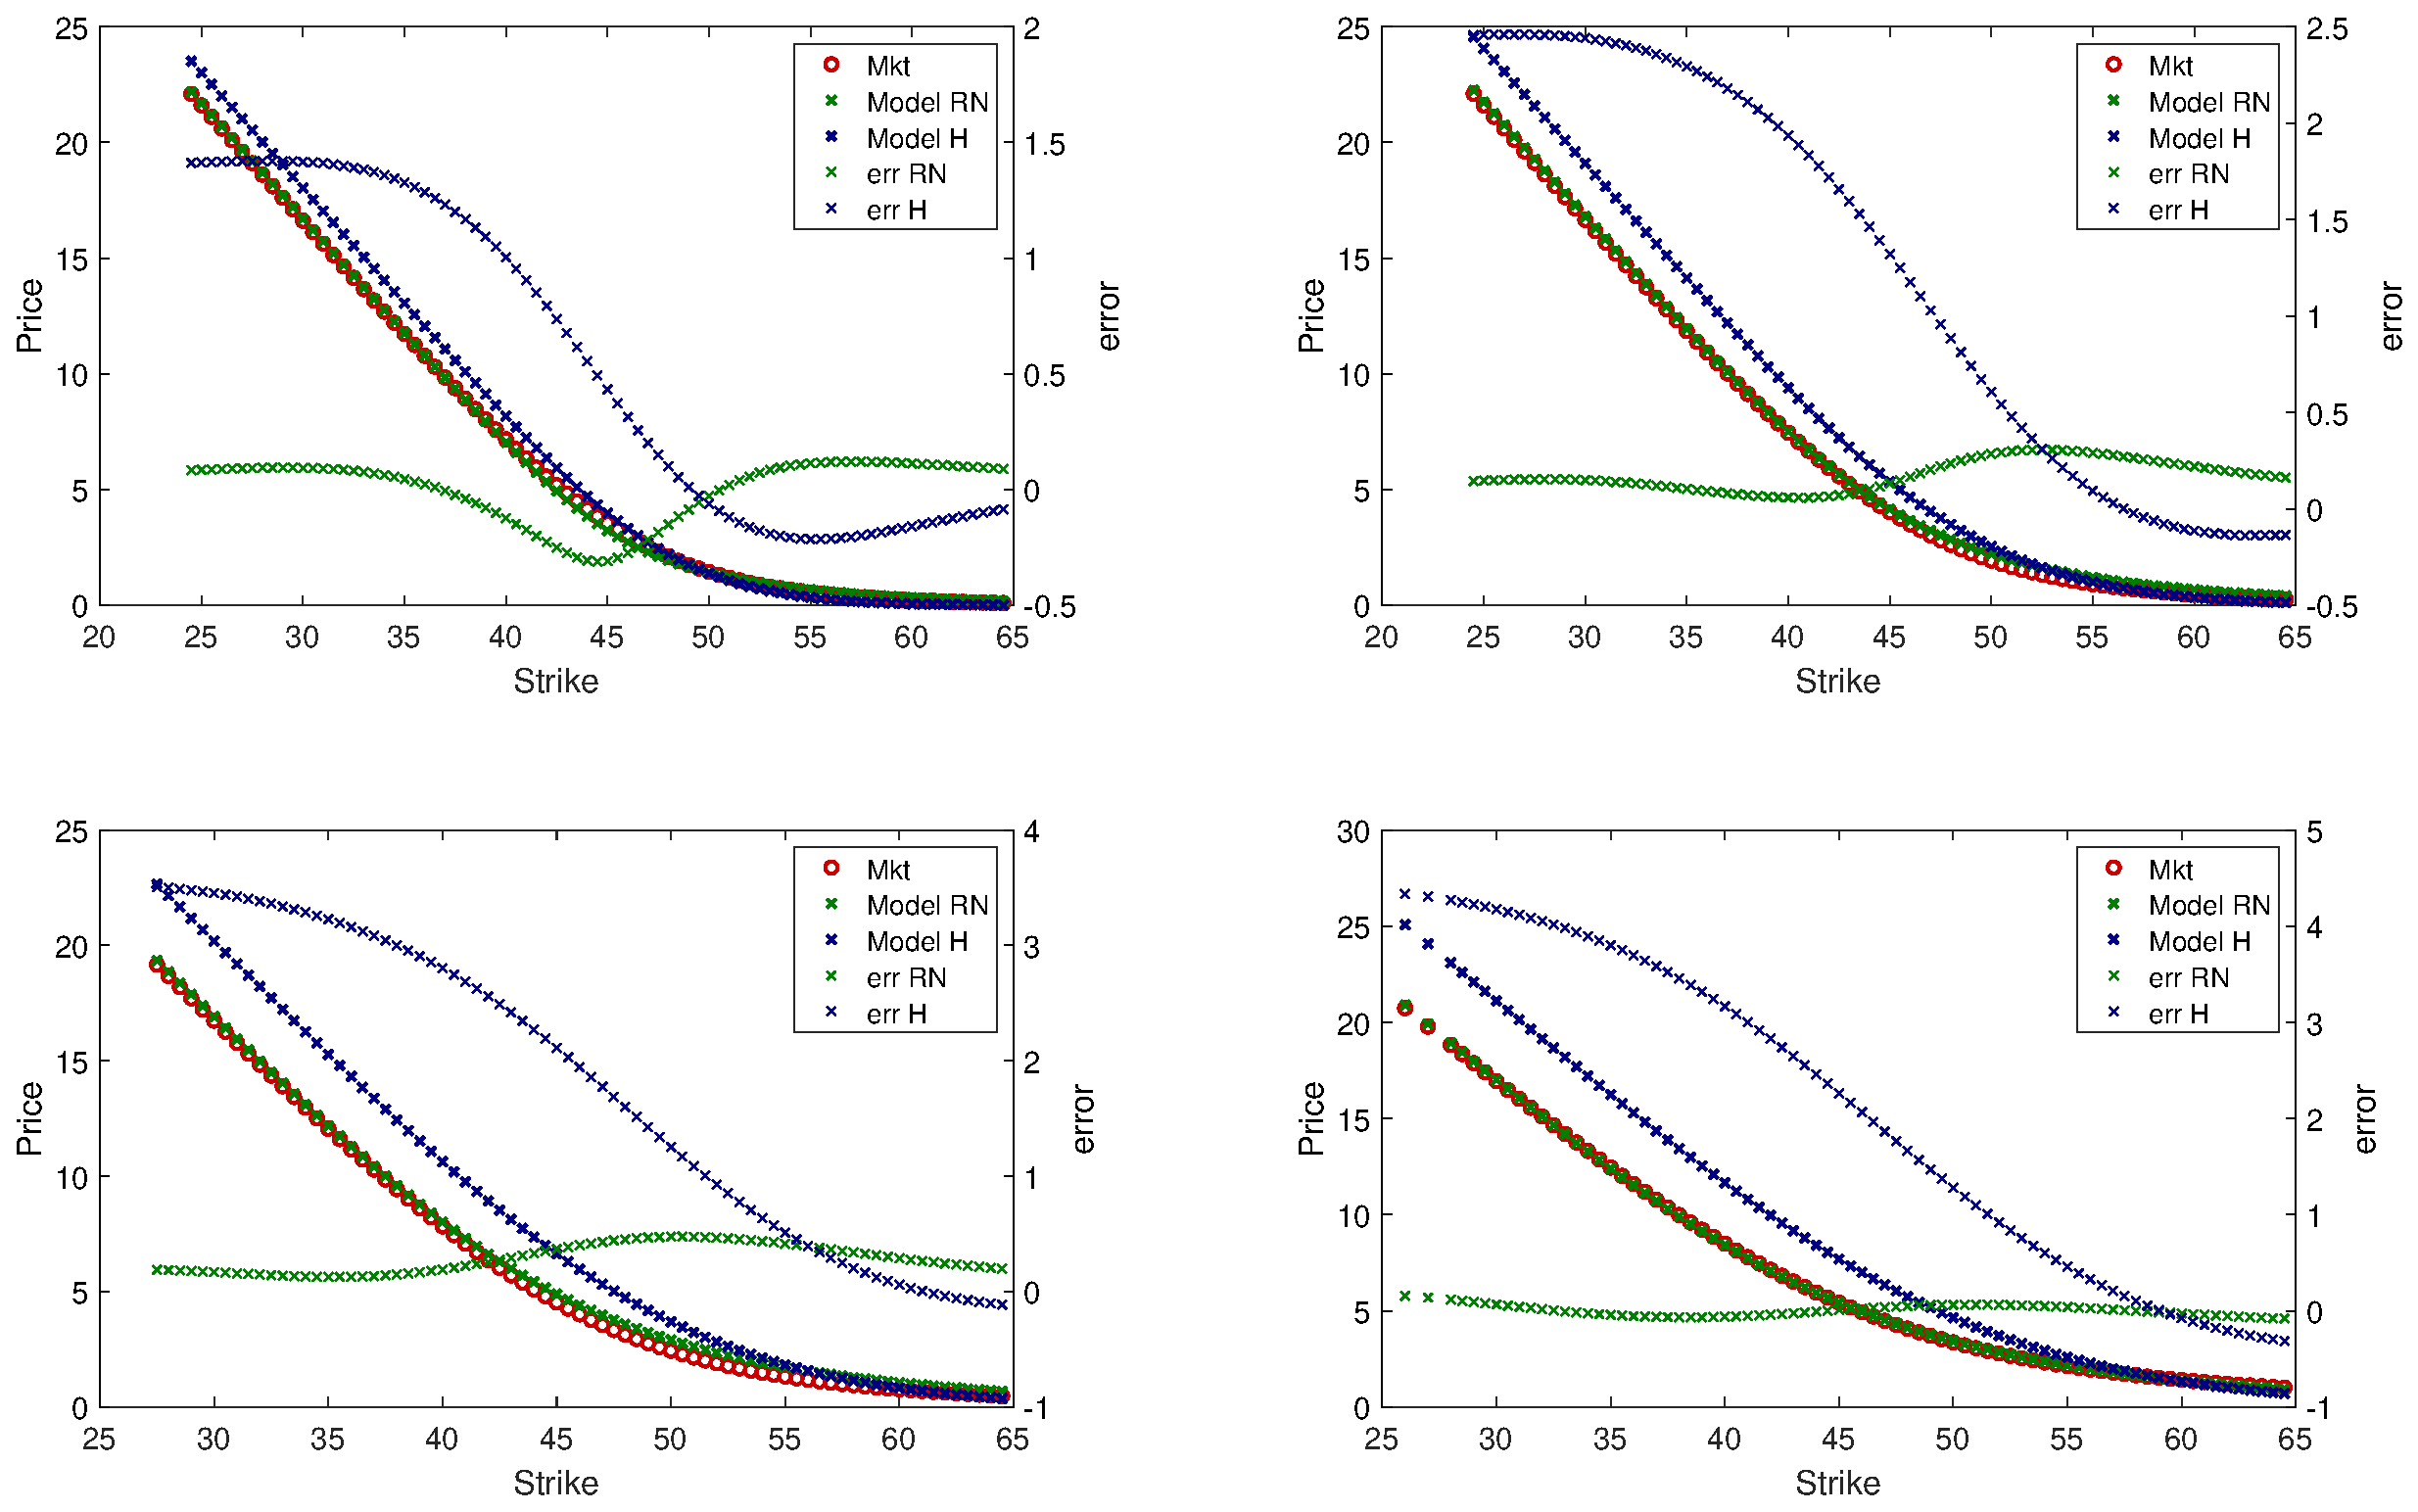
\includegraphics[scale=0.18]{images/MktRepricingHvsRN.eps}
		\caption{Market Repricing for different maturities: observe that historical calibration and Risk-Neutral calibration leads to different parameters and hence to different derivative pricing.}
	\end{figure}
	
	
\end{frame}

%----------------------
% SLIDE
%----------------------
\begin{frame}
	\frametitle{Numerical Application - Risk-Neutral Calibration}	
	\begin{figure}
	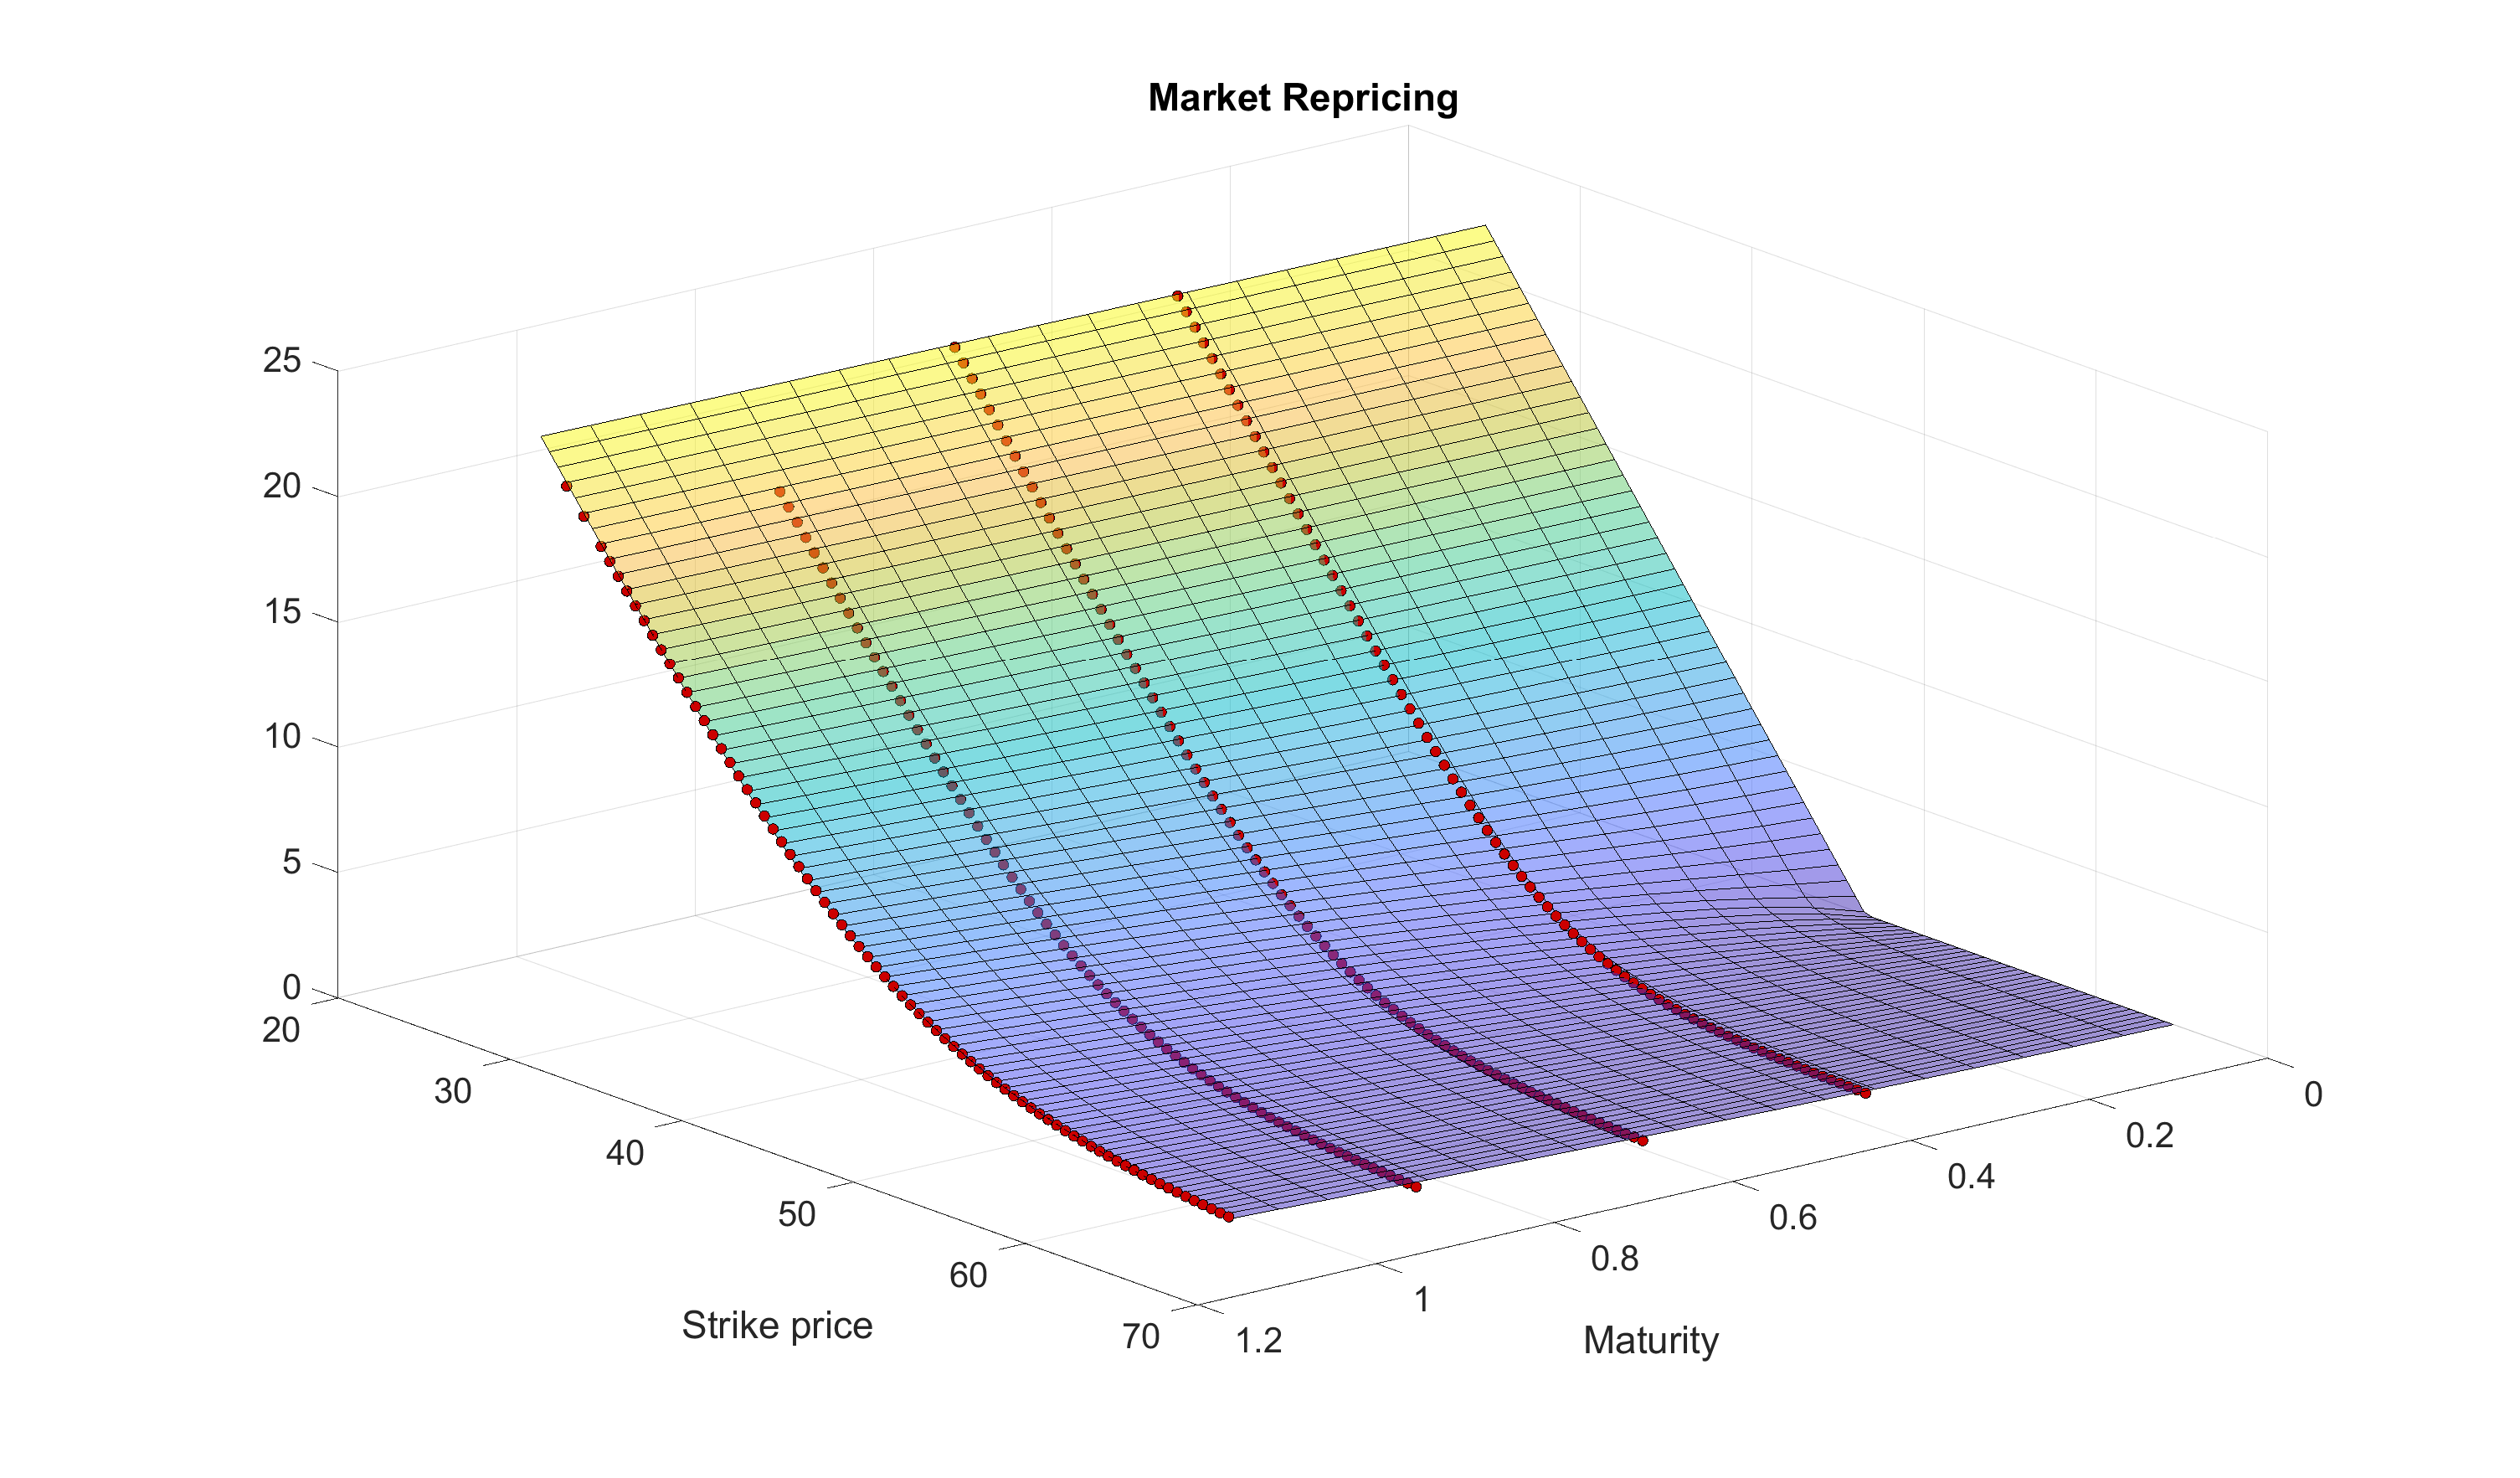
\includegraphics[scale=0.2]{images/RepricingPlot.eps}
	\caption{Market repricing using Risk-Neutral parameters.}
\end{figure}
\end{frame}

%----------------------
% SLIDE
%----------------------
\begin{frame}
	\frametitle{Numerical Application - Risk-Neutral vs Historical}	
\begin{mybox}{darkgreen}{\textbf{Important remark}:}
\quotes{Never} use historical calibration for derivative pricing! The obtained prices are not coherent with the ones observed in the market!
\end{mybox}
\vspace{0.5cm}
\textbf{Q}: Why \quotes{never}? If the derivative market is not liquid the only reasonable idea is to use parameters from historical calibration for derivatives pricing.

\vspace{0.5cm}
\begin{mybox}{darkgreen}{\textbf{Why Variance Gamma model?}}
	Why Variance Gamma model, in this case, is preferred to the original Black-Scholes model?
\end{mybox}


\end{frame}


%----------------------
% SLIDE
%----------------------
\begin{frame}
\frametitle{Numerical Application - Volatility smiles}	
	\begin{defn}[Implied volatility]
	In financial mathematics, the implied volatility of an option contract is that value of the volatility of the underlying instrument which, when input in an option pricing model (such as Black–Scholes), will return a theoretical value equal to the current market price of said option. 
	\end{defn}
	
	Black-Scholes model assumes that the volatility is constant. But, if you retrieve the implied volatility from quoted option prices varying the strike price you get something strange...
	
	
\end{frame}


%----------------------
% SLIDE
%----------------------
\begin{frame}
	\frametitle{Numerical Application - Volatility smiles}	
	
	\begin{figure}
		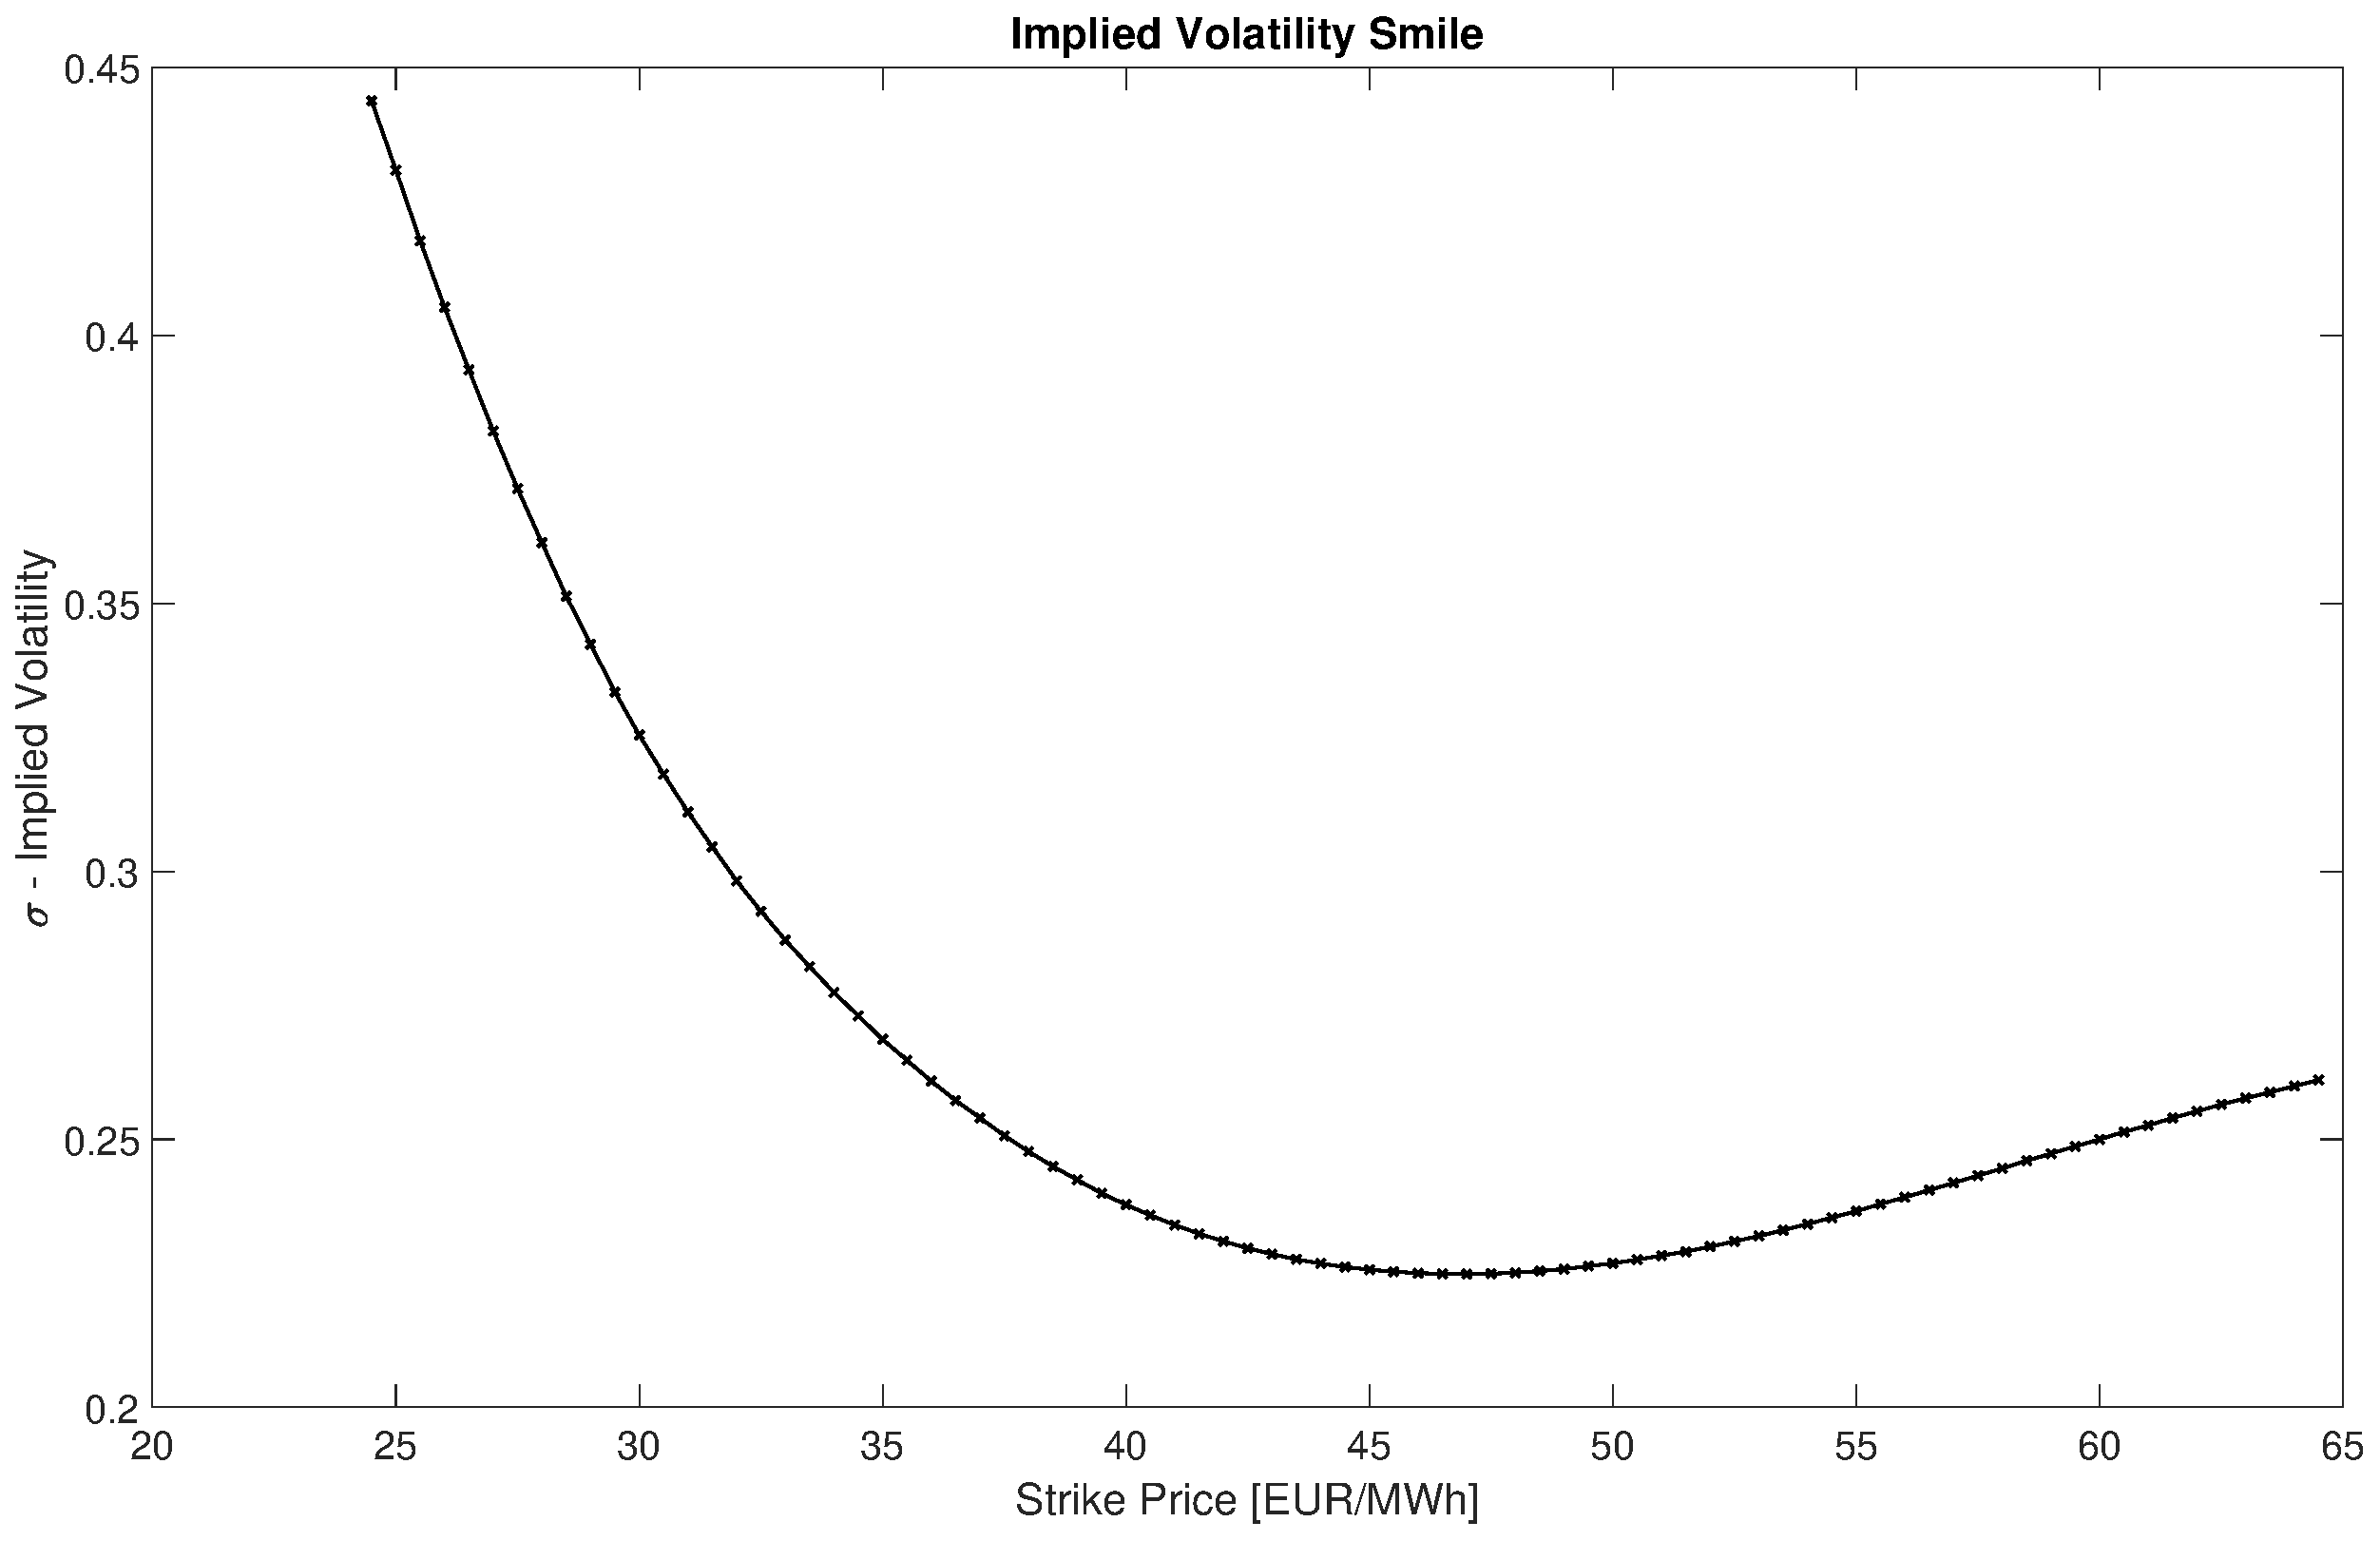
\includegraphics[scale=0.25]{images/VolatilitySmile.eps}
		\caption{Volatility smile varying the strike price $K$, same maturity $T$.}
	\end{figure}
	
	
	
\end{frame}



%----------------------
% SLIDE
%----------------------
\begin{frame}
	\frametitle{Numerical Application - Volatility surface}	
	\begin{figure}
	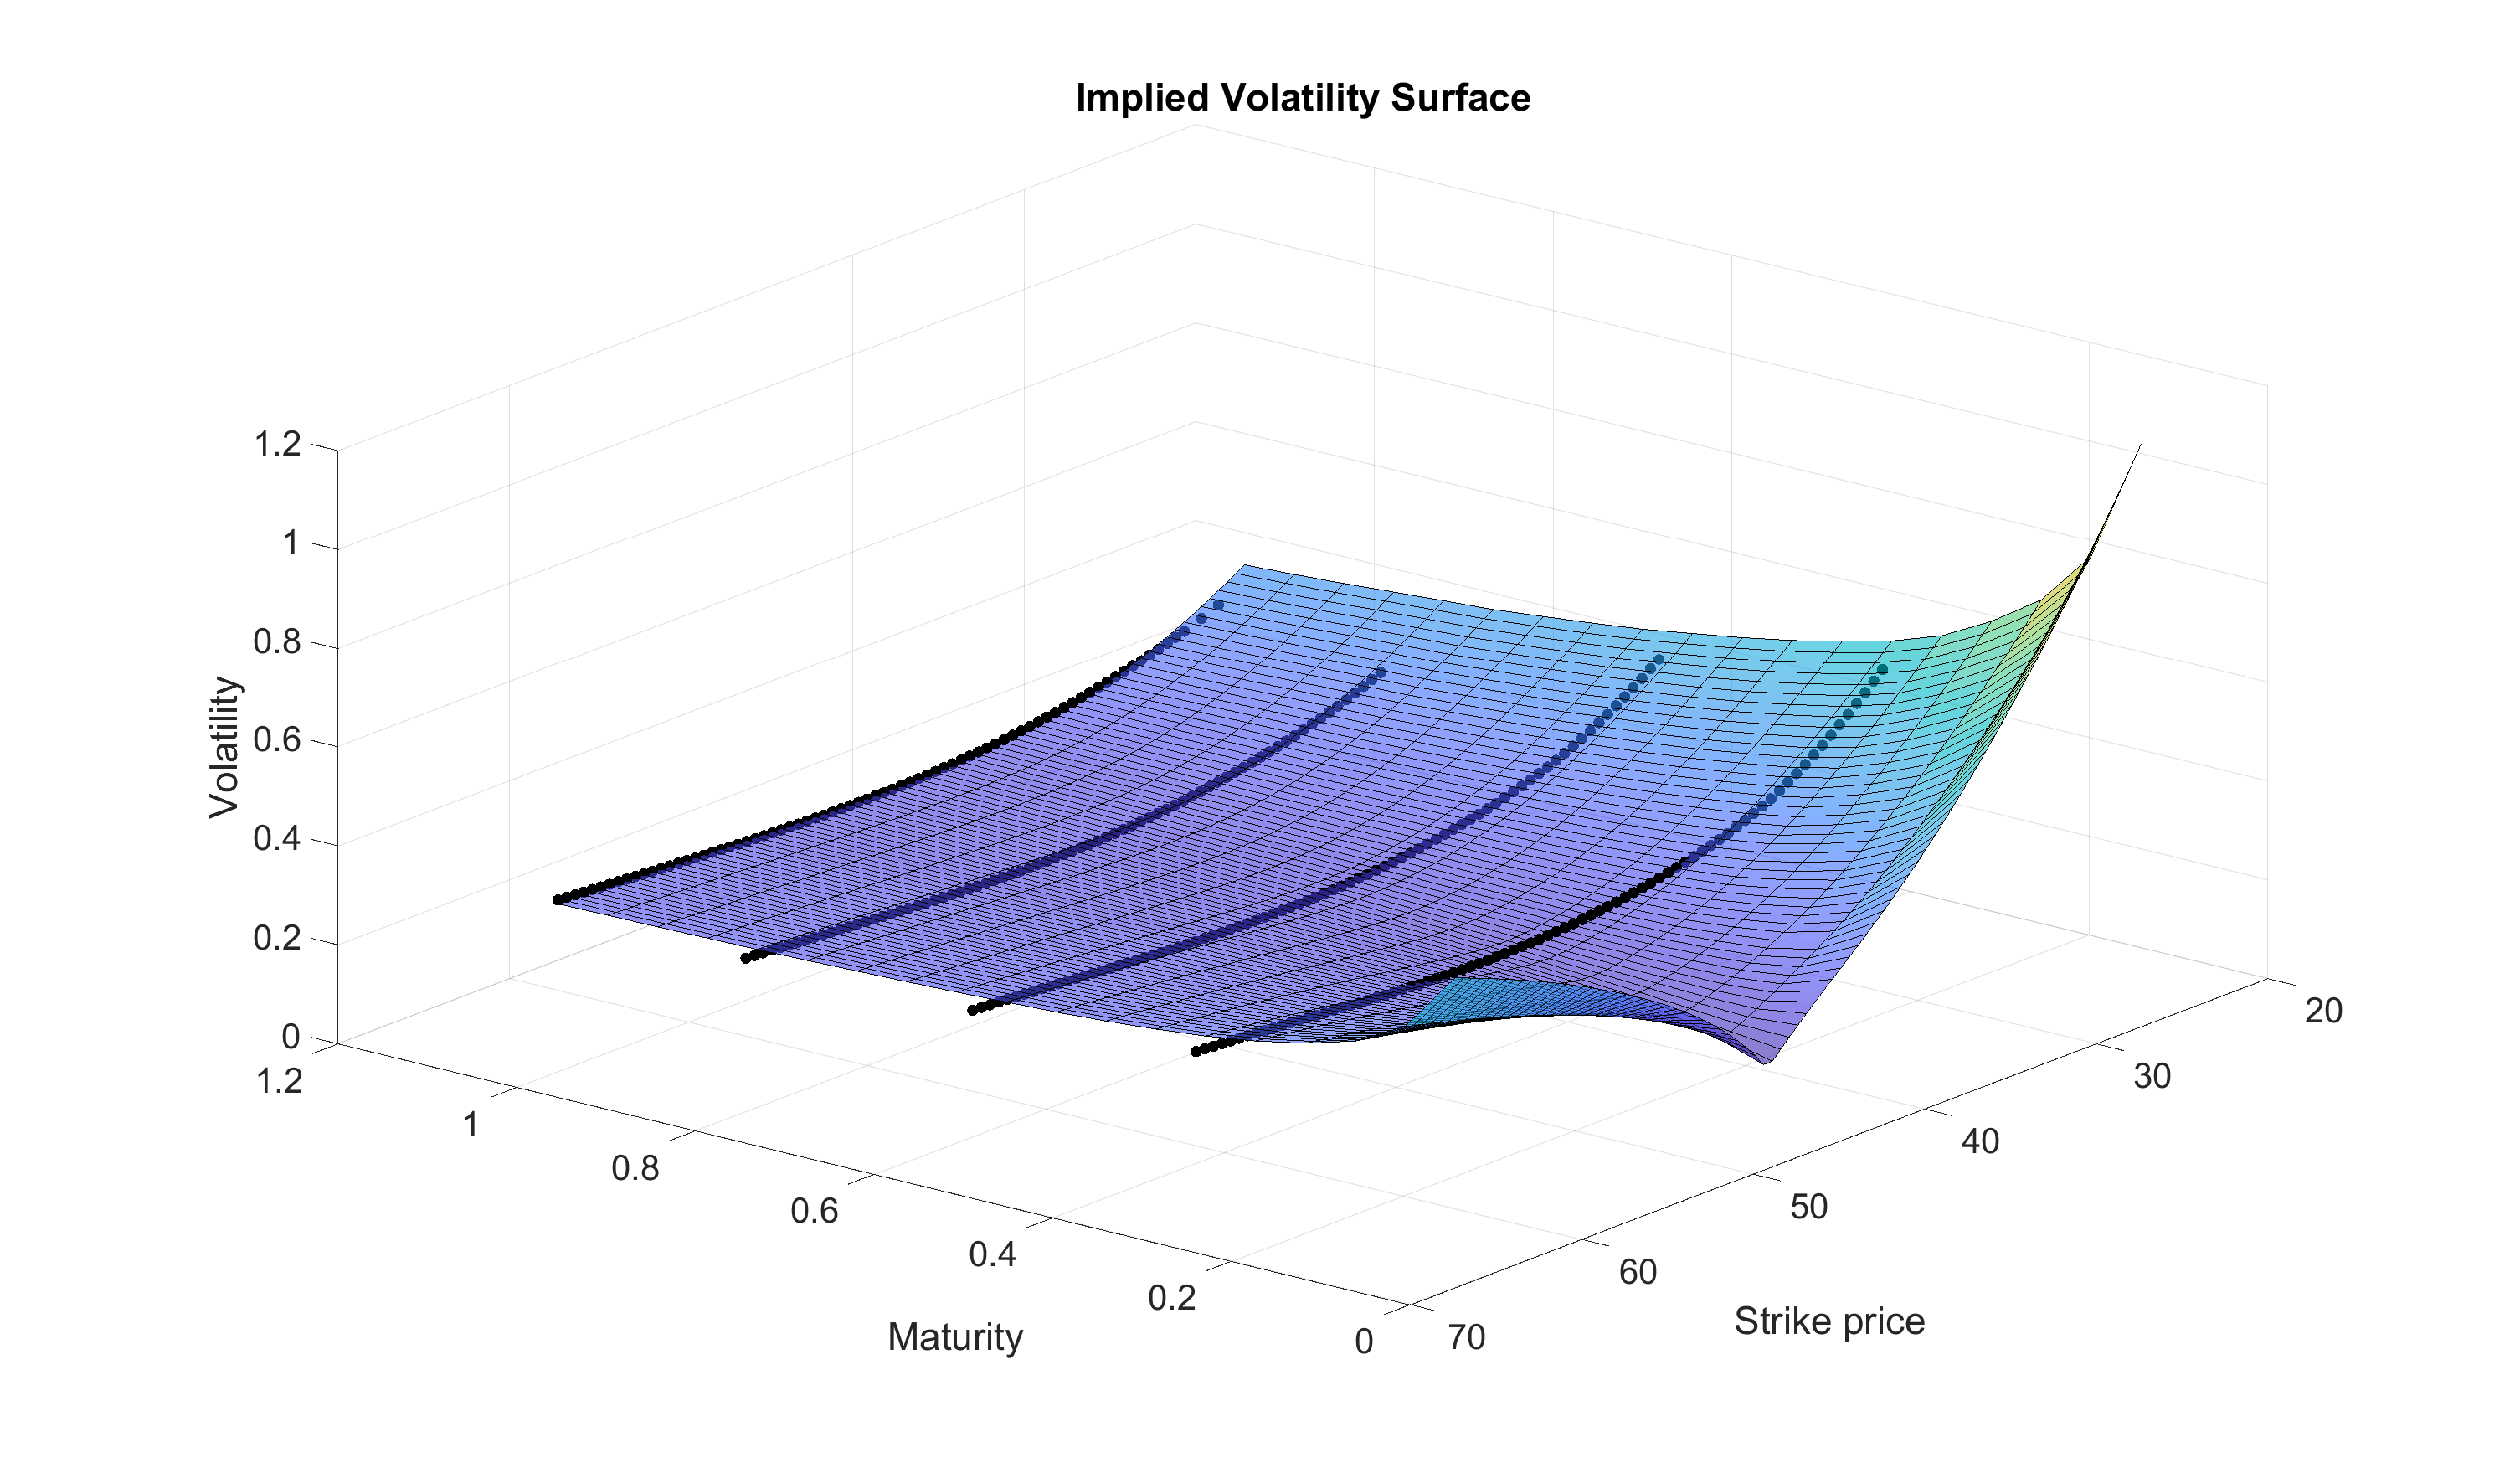
\includegraphics[scale=0.23]{images/surfacePlot.eps}
	\caption{Volatility surface generated by the Variance Gamma model. It is able to fit the implied market volatility. Unlike the Black-Scholes model the volatility is no more constant.}	\end{figure}
\end{frame}



%----------------------
% SLIDE
%----------------------
\begin{frame}
	\frametitle{Numerical Application - Volatility surface}	
	\begin{mybox}{darkgreen}{\textbf{Conclusions}}
		\begin{itemize}
			\item Risk-Neutral calibration of Variance Gamma process is easy since a semi-analytic option pricing formula for Vanilla option is available.
			\item Log-returns distribution it is not Gaussian and fits better the market one.  
			\item The volatility is not constant and volatility smiles can be replicated by the model.
			\item Some important market features can be modeled by simply adding one more parameter ($\nu$) with respect the original Black-Scholes model.
		\end{itemize}
		
		\end{mybox}
\end{frame}


%----------------------
% SLIDE
%----------------------
\begin{frame}[allowframebreaks]
\frametitle{Bibliography}
\bibliographystyle{plainnat}
\bibliography{biblioAll}
\end{frame}
%----------------------------------------------------------------------------------------

\end{document}